% !TEX root = ../Thesis.tex
\chapter{Evaluation}

In this section we want to talk about the evaluation as a whole. We want to look at the phrases we took, how we carried it out, the results observed and compare it to other results.

\section{MacKenzie Phrase Set}
One precondition for the evaluation is to use the MacKenzie Phrase Set\footnote{http://www.yorku.ca/mack/PhraseSets.zip}. Basically, this is just a set of 500 phrases. According to the paper \cite{10.1145/765891.765971}, such a phrase set should use phrases of moderate length, that are easy to remember and representative for the target language. These phrases do not contain any punctuation. Some of them use uppercase characters, but the authors mention, that participants can also be instructed to ignore the case of the characters. 
%The complete MacKenzie Phrase can be downloaded at \hyperlink{http://www.yorku.ca/mack/PhraseSets.zip}{http://www.yorku.ca/mack/PhraseSets.zip}.
\\
Some statistics for the whole phrase set, also found in the original paper \cite{10.1145/765891.765971}: The MacKenzie phrase set consists of 500 phrases, that have a minimum length of 16, a maximum length of 43 and an average length of 28.61 characters. On the whole, 2712 words were used, which consist of 1163 unique words. A phrase consists of a minimum of 1, a maximum of 13 and on average of 4.46 words.

\section{Task of the Participants}
The task of the participants is to copy 15 ``random'' phrases. They are not really random, but adjacent phrases from the downloadable MacKenzie Phrase Set (\url{http://www.yorku.ca/mack/PhraseSets.zip}). As they are not in a specific order, e.g. alphabetic order, we decide to do it like this.\\
TODO: PICTURE OF EVALUATION SCENE.
The participants see two text fields. On the top is the phrase to copy, on the bottom the words/phrase they write. If the given phrase matches the user inputted phrase, a sound sounds, such that the participants know when they finish one specific phrase. After that, a new phrase appears until 15 phrases are correctly inputted. If an incorrect word is entered, the user either can use the word suggestions (fig \ref{fig:write_suggestions}) or delete the wrong word and try to write it again. If a mistake is only noticed later on, the participants have to remove all words and characters up to and including the wrong word by using the backspace button.
\label{sec:eva_task}
After this first step, in the second step, we briefly explain two functions of the keyboard, which they can test afterwards. First the scaling buttons and then the function to add a new word. This is important, because we want to know if they find these functions useful and well implemented.\\
The last step of the evaluation is to fill a questionnaire. First it has some general questions about the participant's experience in VR. Then there is a block of twelve questions. The first ten are from the system usability scale and the last two are for the previously mentioned functions they test. Per question, there are five possibilities to set the cross. From 1 (strongly disagree) to 5 (strongly agree). The questions are structured in such a way, that if the user is highly satisfied with everything, they would alternately make a cross at the 5 and 1. TODO: questionnaire as appendix.

\section{Carry-out}
To carry out the evaluation, we used two different VR systems. One was a setup with a HTC vive and HTC vive controllers. The other one included an Oculus Rift headset with corresponding controllers. Even though these are two different systems, it did not change much for the participants. In fact, only the controllers and their buttons differ a bit.\\
To find participants, we wrote an email to students from our university, and asked family members and friends. All in all, eleven people got in touch with us and participated at our evaluation. Every participant got the same explanation to give everybody the same foundation of knowledge.\\
We told them that if they are close enough to the keyboard, then the color gets a bit brighter, and they are in the keyboard's hitbox. We said, the keyboard is movable, if they press and hold the controller's grip button in the hitbox of the keyboard. If they release it, the keyboard gets static again and stays where it got put.\\
To write, they do also have to be in the hitbox of the keyboard but not pressing and holding the grip button, but the trigger button. Then they have to make a gesture over the characters of the keyboard to write a word. We also told them, that if they do a full gesture and a word longer than one character is written, a space is automatically put behind the word. We also said to them, that single characters could be inputted by clicking on a key of the intended character. If they did so, no space is put, and they have to do it on their own. In the English language, this is particularly important for the words ``I'' and ``a''.\\
We also told them, that if they made a gesture and a word was written, there may be one to four other choosable words. They could pick from them, if the word written in the text field is the wrong one. We especially mentioned the word ``the''. All the time ``thee'' would be written as the best match, therefore they would have to correct it every time.\\
They were also informed about the backspace. So, that if they use the backspace button after writing a word, the whole word gets deleted and afterwards only single characters get deleted.\\
We also told the participants, that we have enough time and that they should not hurry, but rather look, that the inputted words are correct. Because if they are not correct, they have to use the backspace a lot of times.

\section{Results}
Now, we want to talk about the results and some statistics we gained through the evaluation.\\

\subsection{System Usability Scale}
First, we begin with the results of the SUS questions. These ten questions were:\\
1. I think that I would like to use this system frequently when I work in VR\\
2. I found the system unnecessarily complex\\
3. I thought the system was easy to use \\
4. I think that I need the support of a technical person to be able to use this system\\
5. I found the various functions in this system were well integrated\\
6. I thought there was too much inconsistency in this system\\
7. I would imagine that most people would learn to use this system very quickly\\
8. I found the system very cumbersome to use\\
9. I felt very confident using the system\\
10. I needed to learn a lot of things before I could get going with this system
\iffalse
\begin{table}[ht!]
    \centering
    \caption{Results from the System Usability Scale (SUS) from the questionnaire (first ten questions)}
    \begin{tabular}{cccc} \toprule
        question&average score&perfect possible score&$\sigma$\\ \midrule
        1 & 4.27 & 5.0 & 0.445\\ 
        2 & 1.09 & 1.0 & 0.287\\
        3 & 4.64 & 5.0 & 0.481\\ 
        4 & 1.27 & 1.0 & 0.617\\
        5 & 4.64 & 5.0 & 0.481\\
        6 & 1.64 & 1.0 & 0.979\\
        7 & 4.64 & 5.0 & 0.481\\
        8 & 1.45 & 1.0 & 0.498\\
        9 & 4.09 & 5.0 & 0.514\\
        10 & 1.55 & 1.0 & 0.656\\
        \bottomrule
    \end{tabular}
    \label{tab:table}
\end{table}
\fi
\begin{figure}[H]
    \noindent
    \makebox[\textwidth][c]{
        \centering
        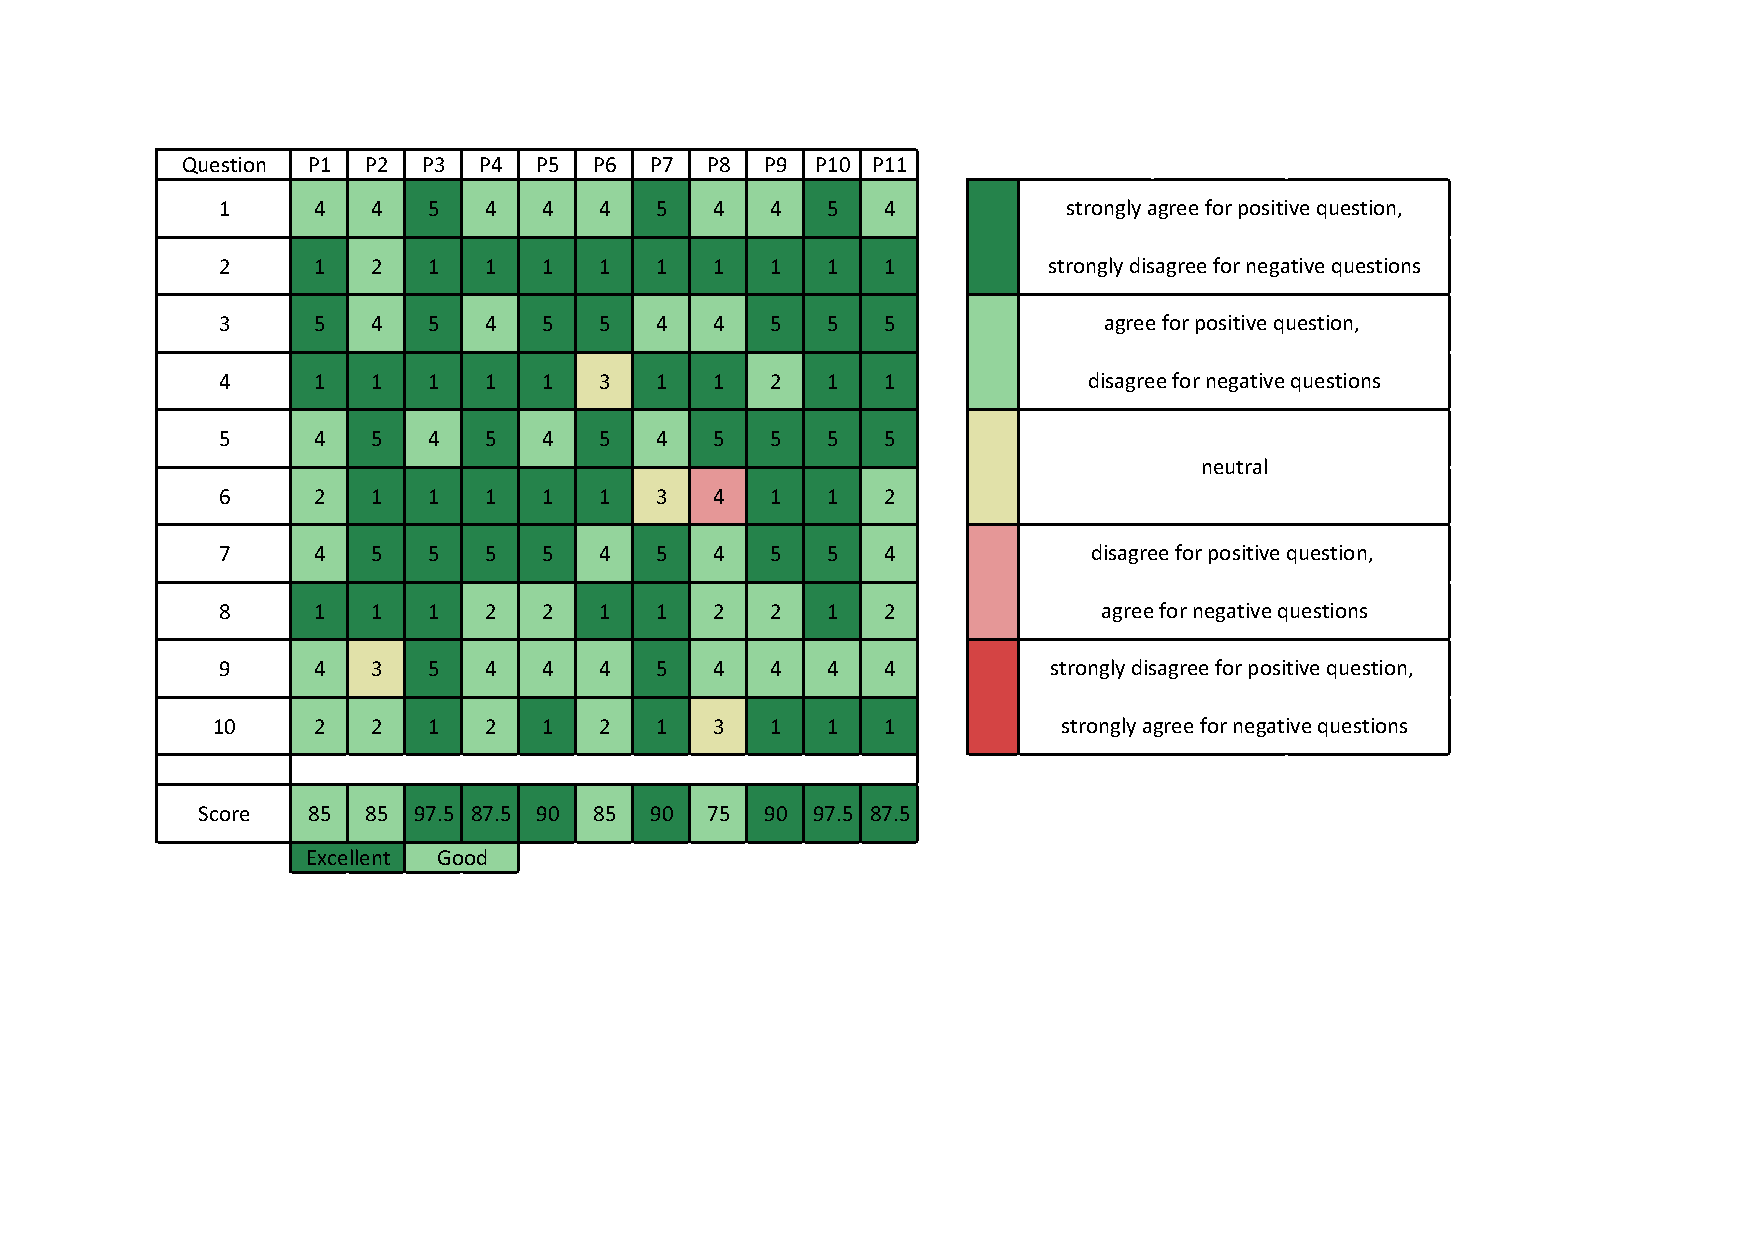
\includegraphics[width=1.3\textwidth]{SUS_scoring.pdf}\hspace{-4em}
    }
    \vspace*{-10em}
    \caption{System Usability Scale with all the given points per question from every participant}
    \label{fig:SUS_score}
\end{figure}

Question 9 got the worst score, but with it being a 4.09 out of 5, it is still pretty good. From these values, we can calculate a usability score. Every question with an even number is a negative one. That means, a score of one or ``strongly disagree'' is the highest possible. For the other questions, a score of five or ``strongly agree'' is the best possible score. So, from the odd numbered questions we have to subtract 1 from the average score. And for the even numbered questions we have to subtract their average score from 5. At the end, we have to sum up these ten newly calculated values and multiply them by 2.5. Our calculated usability score is 88.18. This is a high score, because from a score of 85.5 points, one talks about an excellent system usability. Therefore, we are really satisfied with the results of this.\\
We do also have two other questions about the scale and the ``add word'' function:\\
11. The function to add words is well implemented and easy to use\\
12. The function to scale the keyboard is unnecessary\\
Question 11 got a score of 4.55 out of 5 and question 12 got a score of 2.18, whereby 1 would be ideal. We conclude from these two questions, that the ``add word'' function makes a good impression whereas the scale function does not perform so well.\\

\subsection{Writing Speed}
One important thing of our evaluation is to find out, how fast users can write with our word-gesture keyboard. As unit to measure these values, we take the ``words per minute'' wpm. We calculate the wpm with following formula: 

\begin{equation}
    WPM = \frac{\mid T \mid}{S} \times 60 \times \frac{1}{5}
\end{equation}
where $T$ is all the phrases a participant had to write, hence $\mid T \mid$ is the number of characters a participant had to write. $S$ is the time in seconds they used to write all 15 phrases.\\

\begin{table}[ht!]
    \centering
    \caption{average wpm, lowest wpm and highest wpm per participant. For the first three, we failed to get all data.}
    \begin{tabular}{cccc} \toprule
        participant&average WPM&lowest WPM&highest WPM\\ \midrule
        1 & 11.457 & - & -\\ 
        2 & 12.19 & - & -\\
        3 & 13.055 & - & -\\ 
        4 & 11.609 & 5.3 & 25.5\\
        5 & 12.578 & 6.83 & 21.65\\
        6 & 10.285 & 5.27 & 19\\
        7 & 12.423 & 6.1 & 24.41\\
        8 & 16.056 & 8.28 & 30.74\\
        9 & 13.363 & 7.96 & 24.15\\
        10 & 17.118 & 7.98 & 24.45\\
        11 & 10.067 & 4.71 & 14.55\\
        \bottomrule
        average&12.75&6.55&23.06\\
        \bottomrule
    \end{tabular}
    \label{tab:WPM}
\end{table}

In Table \ref{tab:WPM} you can see how fast in average the participants were able to write their 15 phrases. We do also list the lowest and highest value. Everything is measured in words per minute.

\begin{figure}[H]
    \centering
    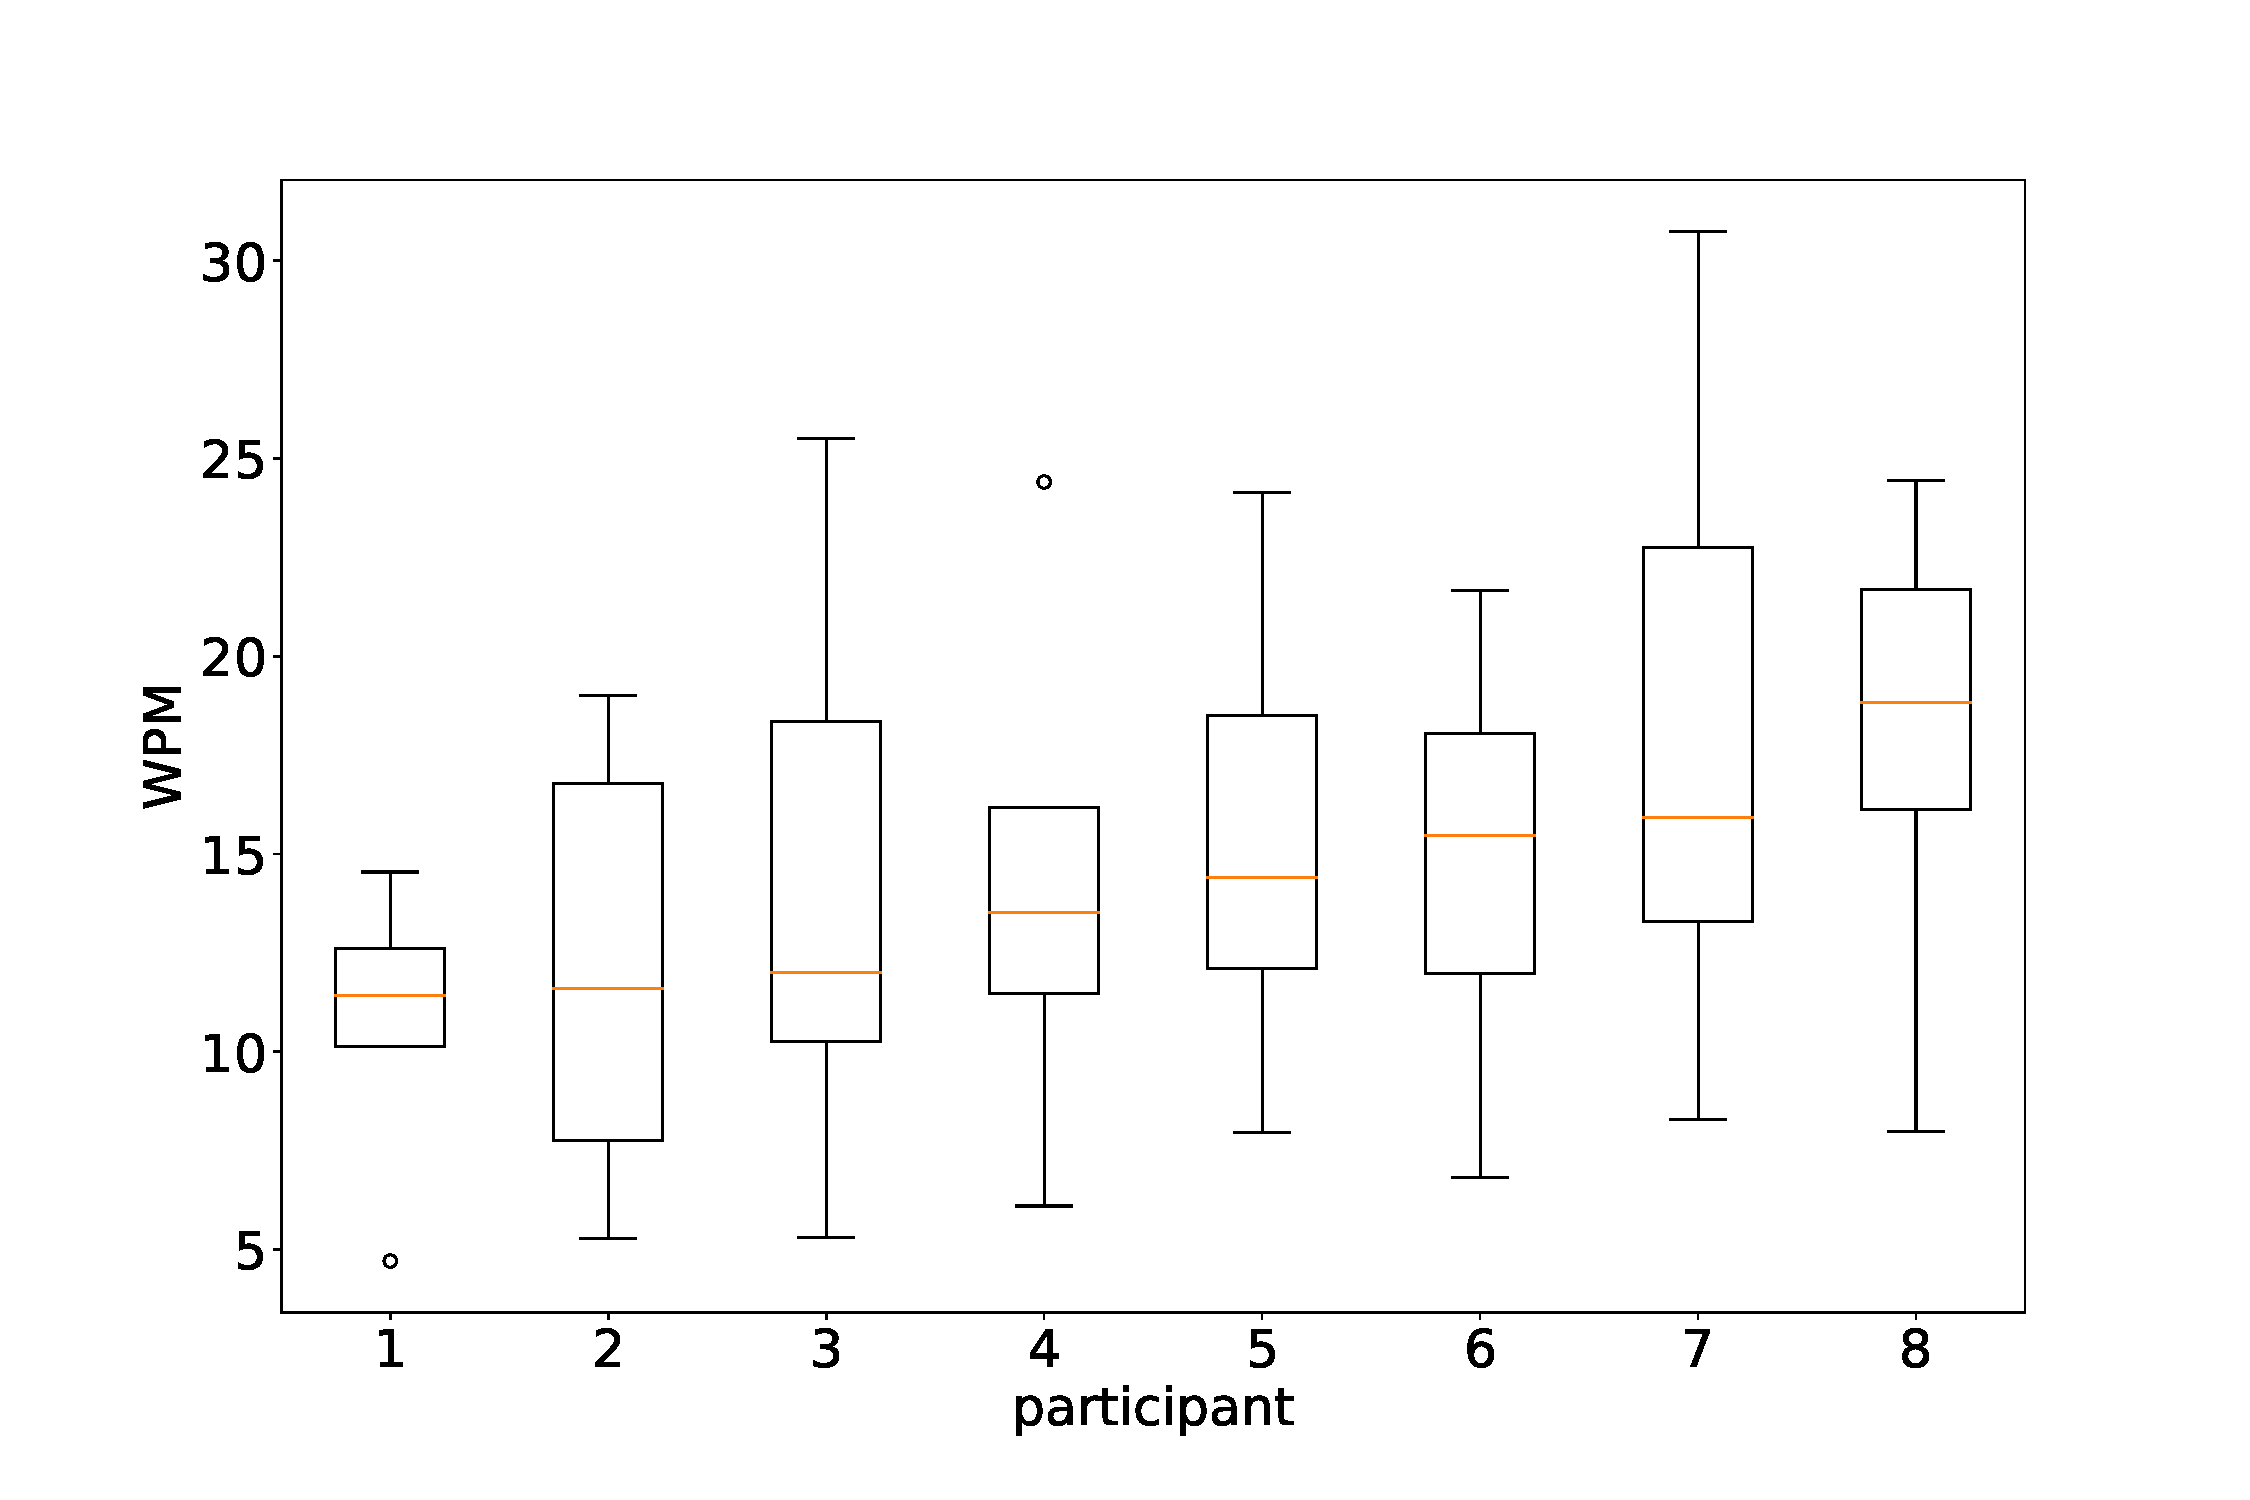
\includegraphics[width=0.9\textwidth]{wpm_boxplot.pdf}
    \caption{for participants 4-11: lowest wpm, 25\% quantile, average wpm, 75\% quantile and highest wpm}
    \label{fig:WPM}
\end{figure}
To understand the values of Table \ref{tab:WPM} a bit better, we make a so-called boxplot for every participant, for whom we have the data. We can see in fig \ref{fig:WPM}, the higher the participant's median, most of the time they do also have higher lowest wpm value. The lowest wpm values mostly come about because a participant made a mistake and had to delete a lot and basically write the phrase two times. On the other hand, most of the highest WPM values come about because a participant made no mistake in writing the phrase. The rectangle in the middle of the two bars shows how consistent or inconsistent a participant's writing speed is. The lower bound is the 25\% quantile, the upper bound the 75\% quantile. This means, if the rectangle is less high, the writing speed is more consistent.\\
We cannot really find anything that combines writing speed and consistency by looking at our measurements.\\

Next, we want to find out, if the writing speed of the users has something to do with their experience in, on one hand VR writing and on the other hand word-gesture keyboards.\\

\begin{figure}[H]
    \centering
    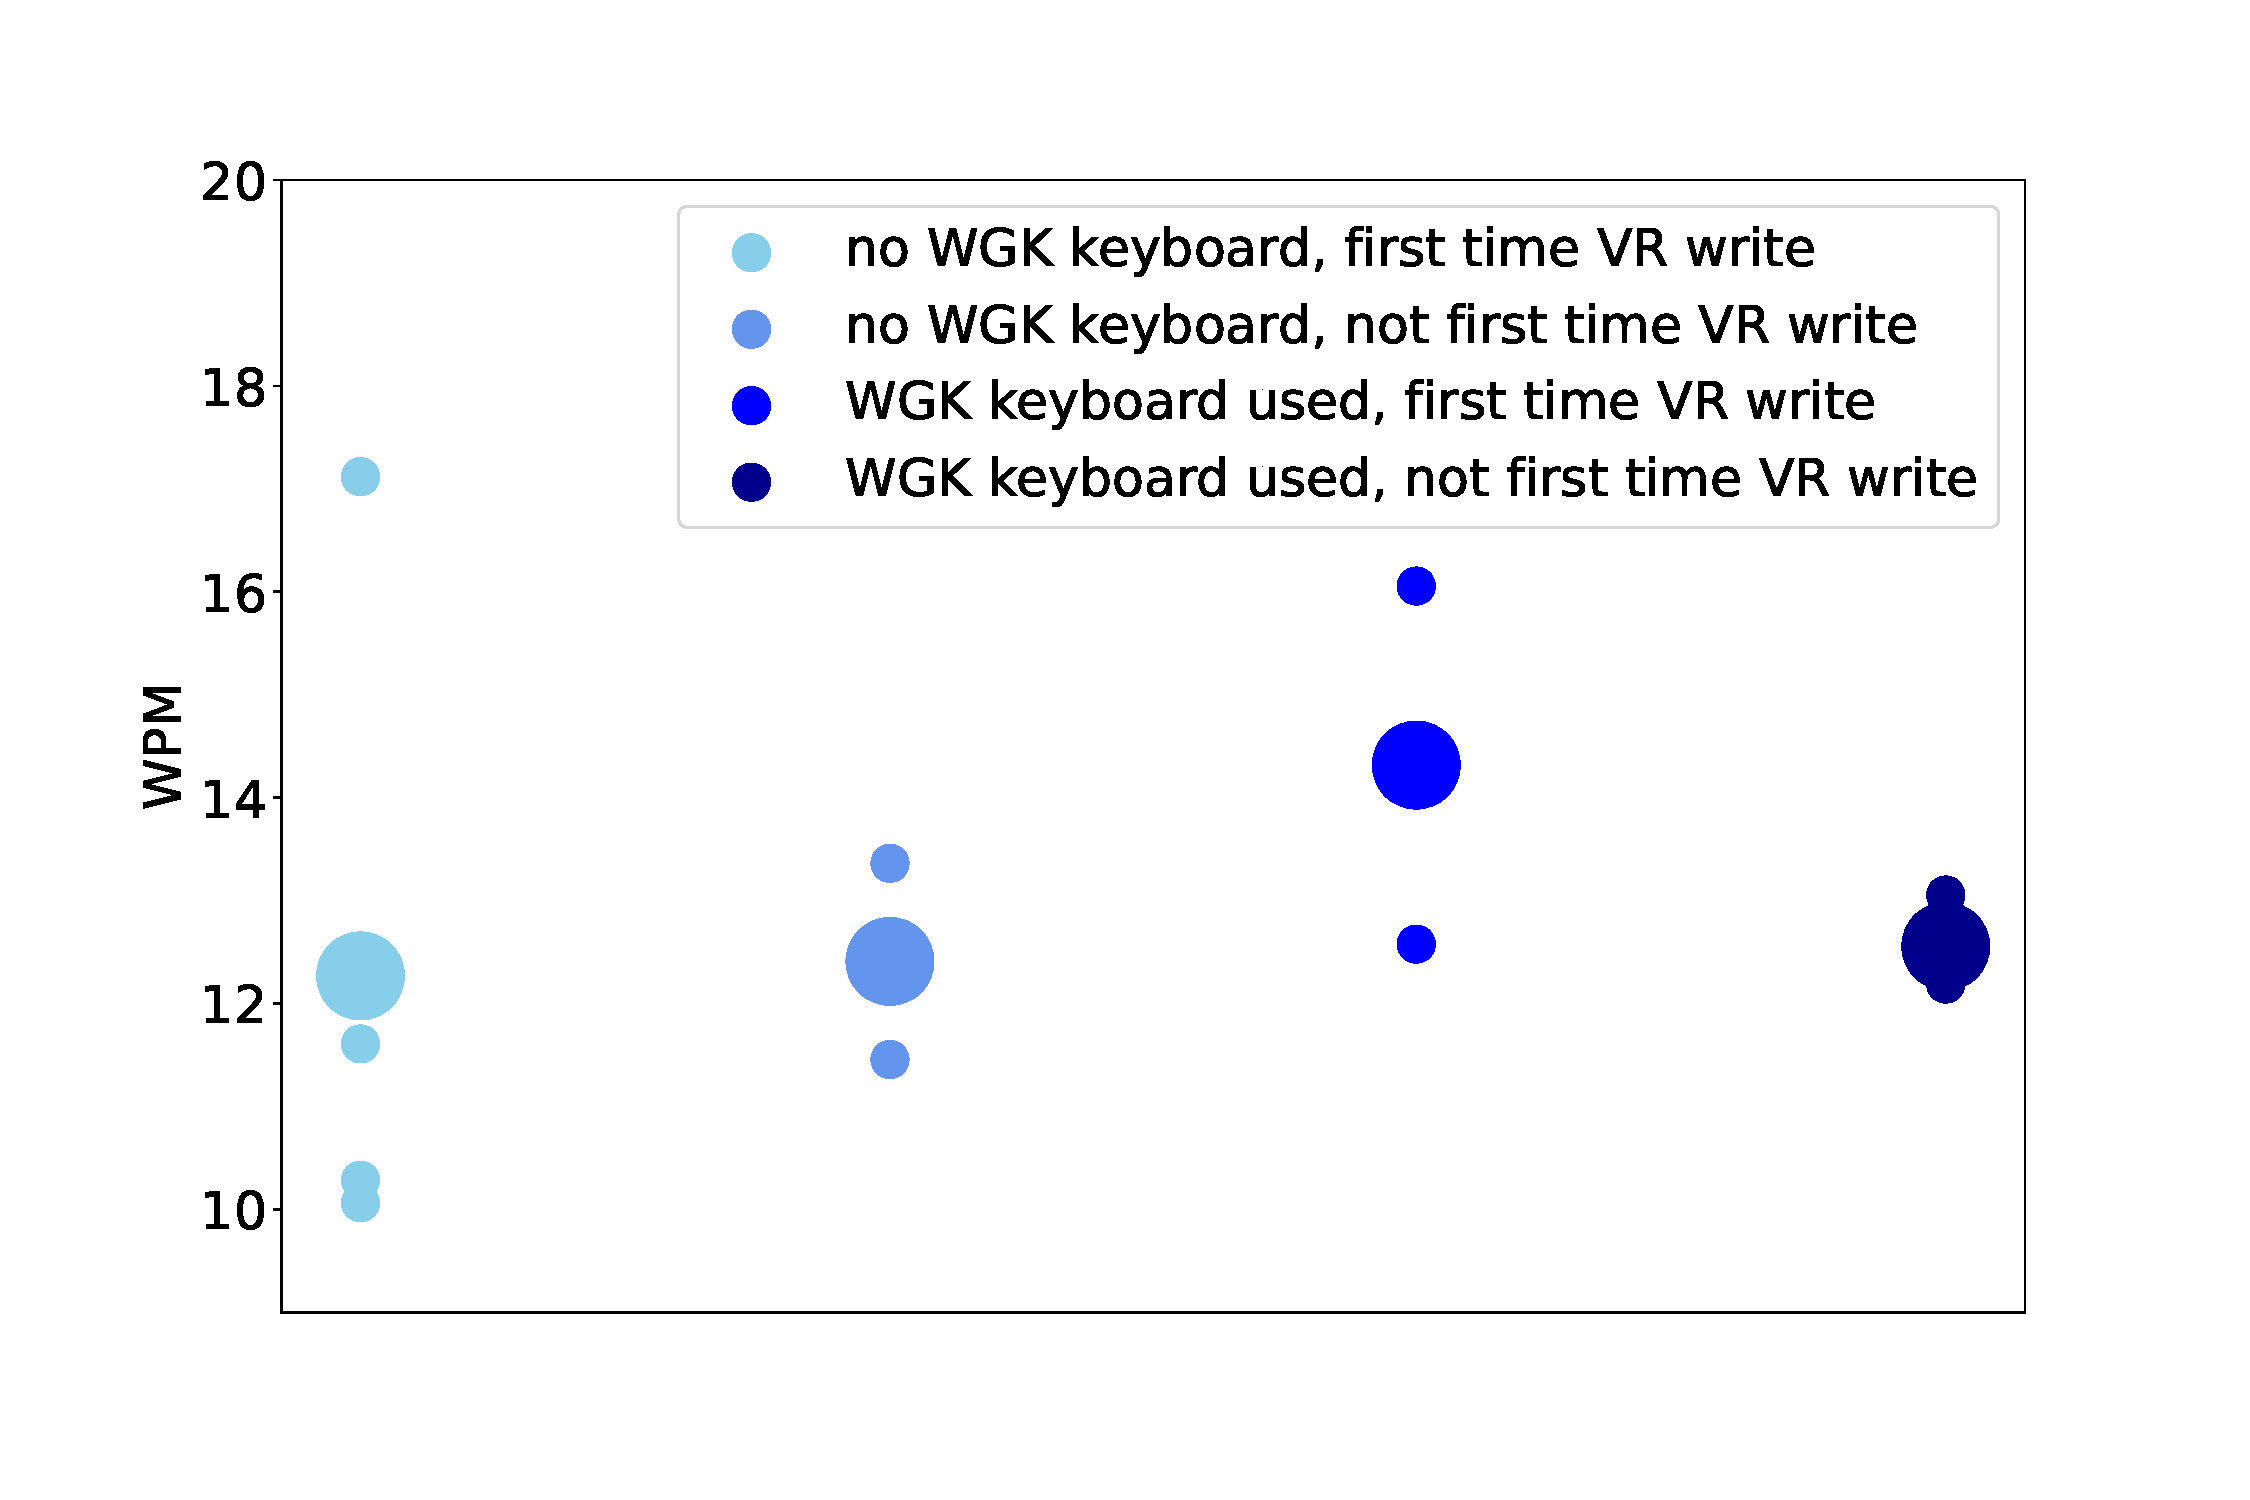
\includegraphics[width=0.9\textwidth]{Comparison_yesno.pdf}
    \caption{Each small dot shows the average wpm for a user. The big dots represent the average wpm per group. The colors are for the different groups of experience in VR writing and word-gesture keyboards}
    \label{fig:WPM_yesno}
\end{figure}

In Fig \ref{fig:WPM_yesno} we can see, that the prior knowledge, that some participants have, did not really help them to write faster. In fact, the fastest group was the one, that is experienced with word-gesture keyboards, but not with writing in VR. But we think due to the small group sizes this is not really presentative. Therefore, we can not conclude much about this, but it could have had a more interesting result.\\

Another thing we wanted to analyze is the writing speed compared to the age:
\begin{figure}[H]
    \centering
    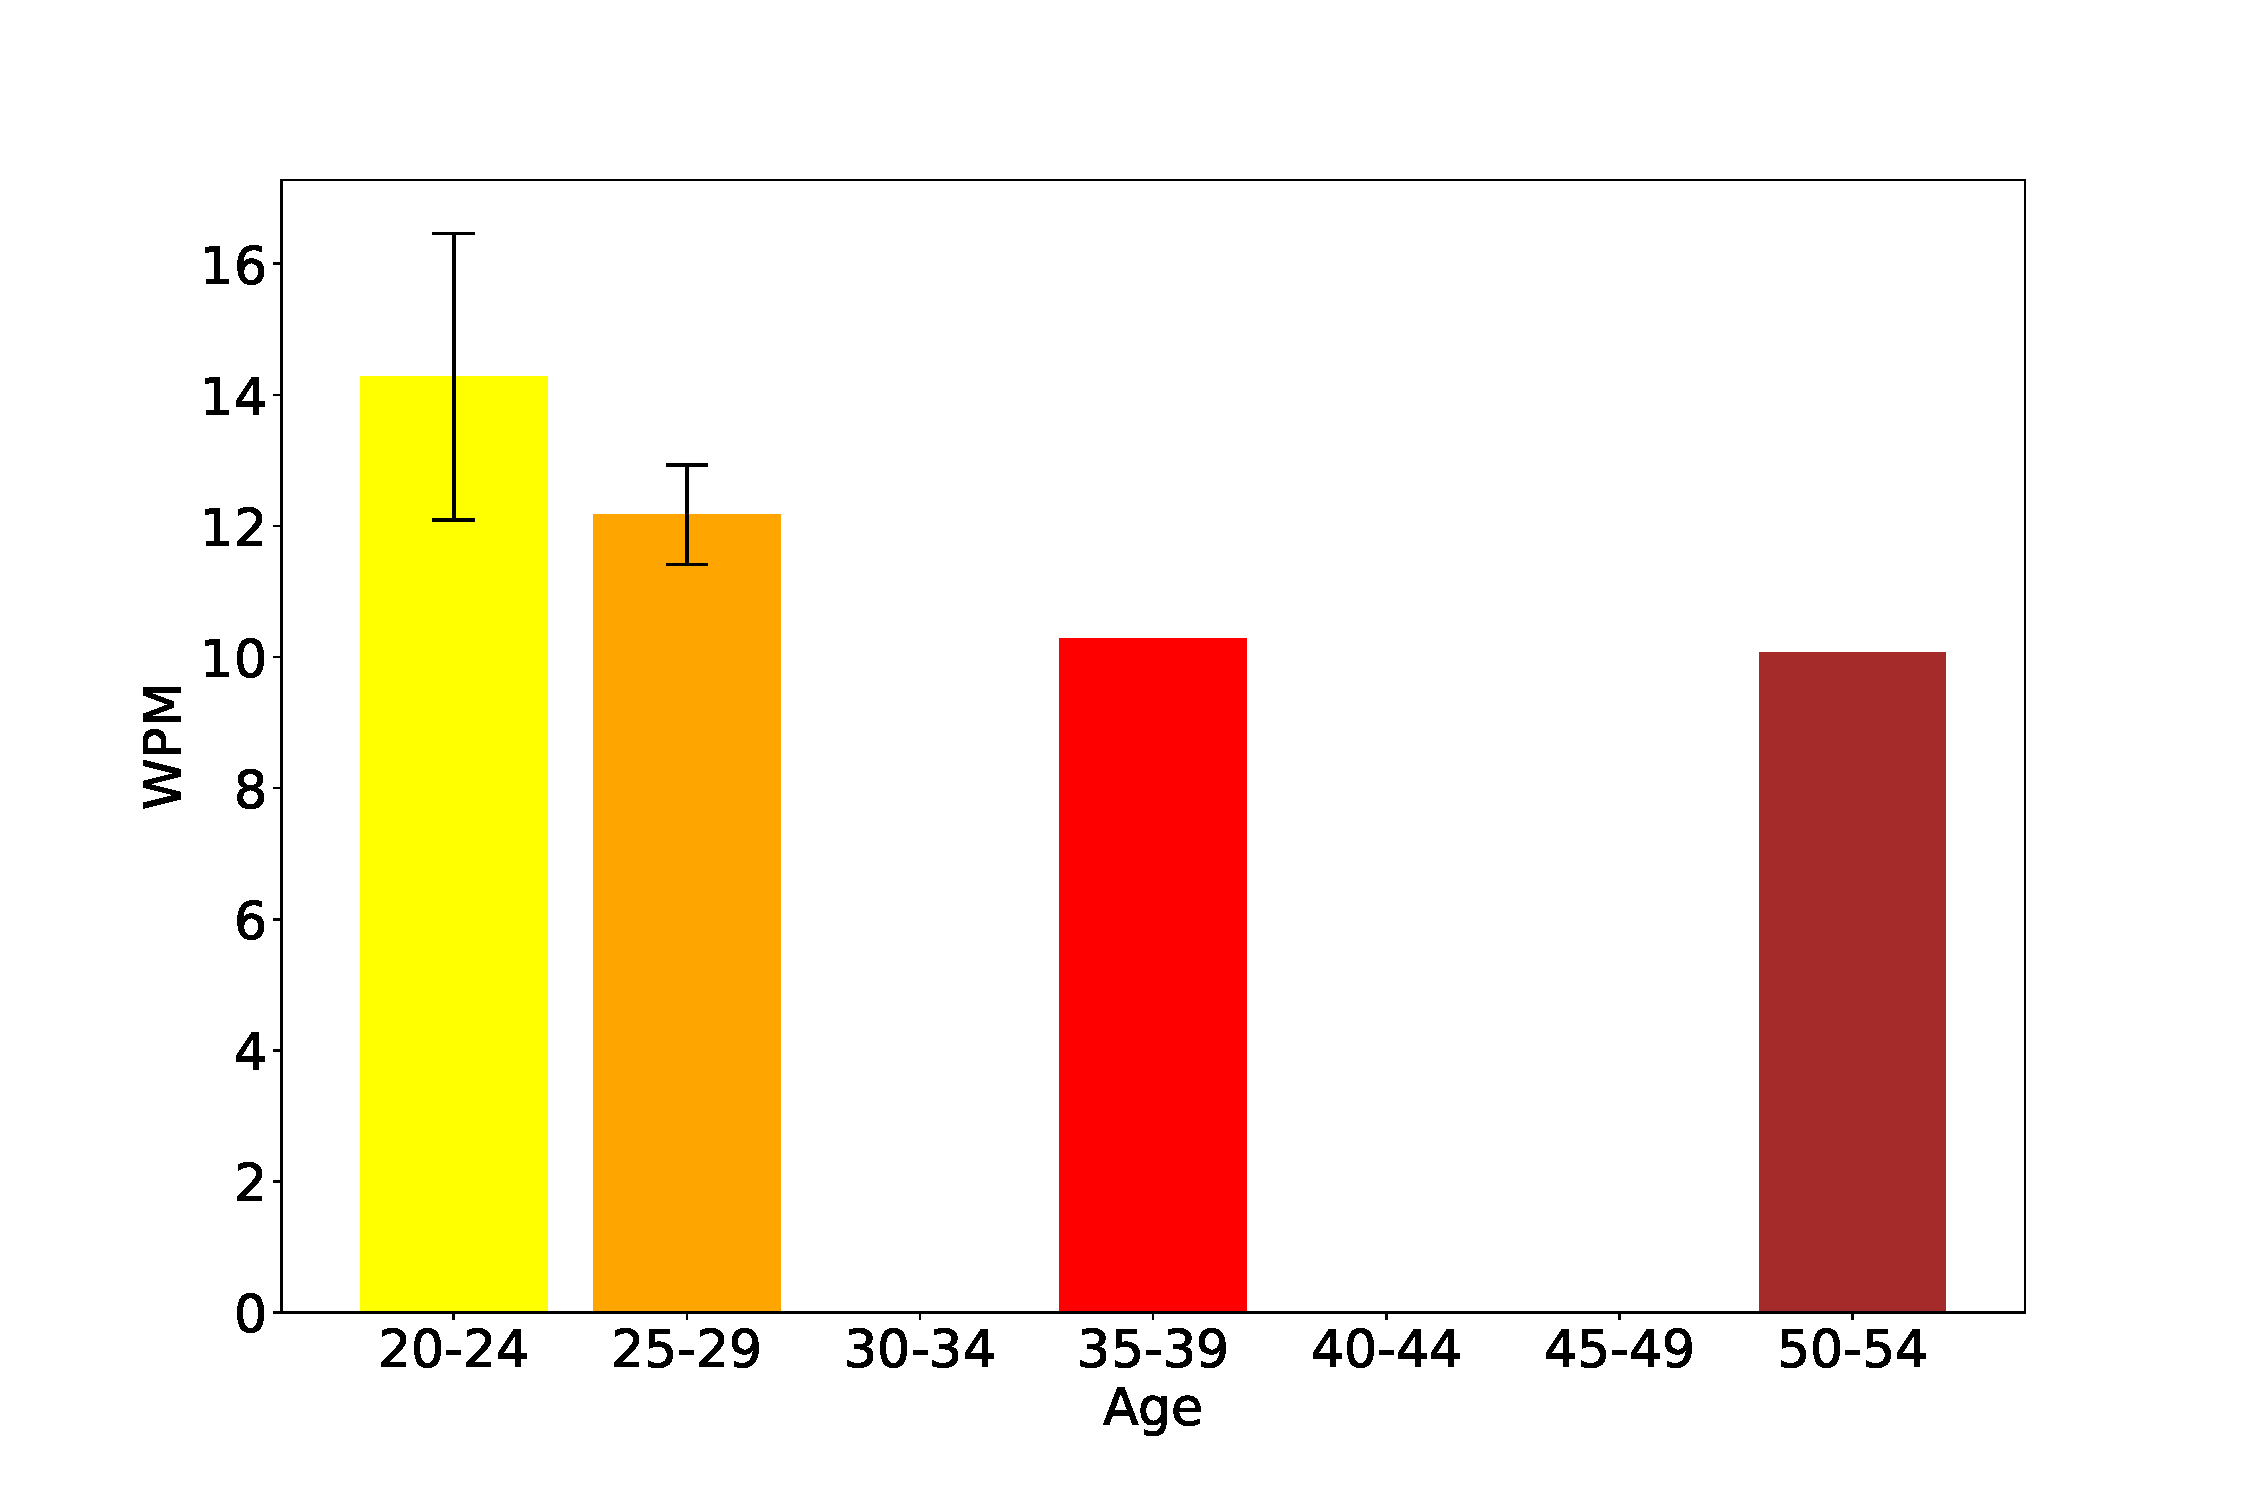
\includegraphics[width=0.9\textwidth]{age_wpm.pdf}
    \caption{wpm values sorted by age groups of five years. The 20-24 and 25-29 groups also have a standard deviation error bar, because they contain of five and four participants. The 35-39 and 50-54 groups do not have an error bar, since each of them only contains of one participant}
    \label{fig:WPM_age}
\end{figure}

We can observe in Fig \ref{fig:WPM_age}, that at least among our participants, the wpm value decreases with the increase in age. This means, the older participants were a bit slower than the younger ones. 

\subsection{Error Rate}
In this section, we will look at different error rates. First of all, we want to find out, which words caused the most errors. Then we investigate some errors caused by the participants. At the end of this section, we take a look at the errors mostly caused by the system's condition.\\

\subsubsection{Most Frequent Error Words}
We looked into all the words that were not the best match, so all the words a participant either corrected or not and also the ones that were not even in the suggestions. The top ten such words are:
\begin{table}[H]
    \centering
    \caption{most frequent error words}
    \begin{tabular}{cc} \toprule
        word&times wrong\\ \midrule
        the & 53\\
        is & 17\\
        to & 14\\
        of & 12\\
        in & 9\\
        for & 8\\
        do & 5\\
        all & 3\\
        more & 3\\
        see & 2\\
        \bottomrule
    \end{tabular}
    \label{tab:error_words}
\end{table}

As we can see in Table \ref{tab:error_words}, the word, that is responsible for most of the errors, is ``the'', which caused 53 errors. In this list, we can also see other words, that could have been avoided by a better implementation. For example ``ìn'' and ``more''.
The best match for these words were ``thee'', ``inn'' and ``moore'', which are words, that do not appear that much in plain language. But we want to go more in depth on this topic later on.

\subsubsection{User and Backspace Error Rate}
\begin{figure}[H]
    \centering
    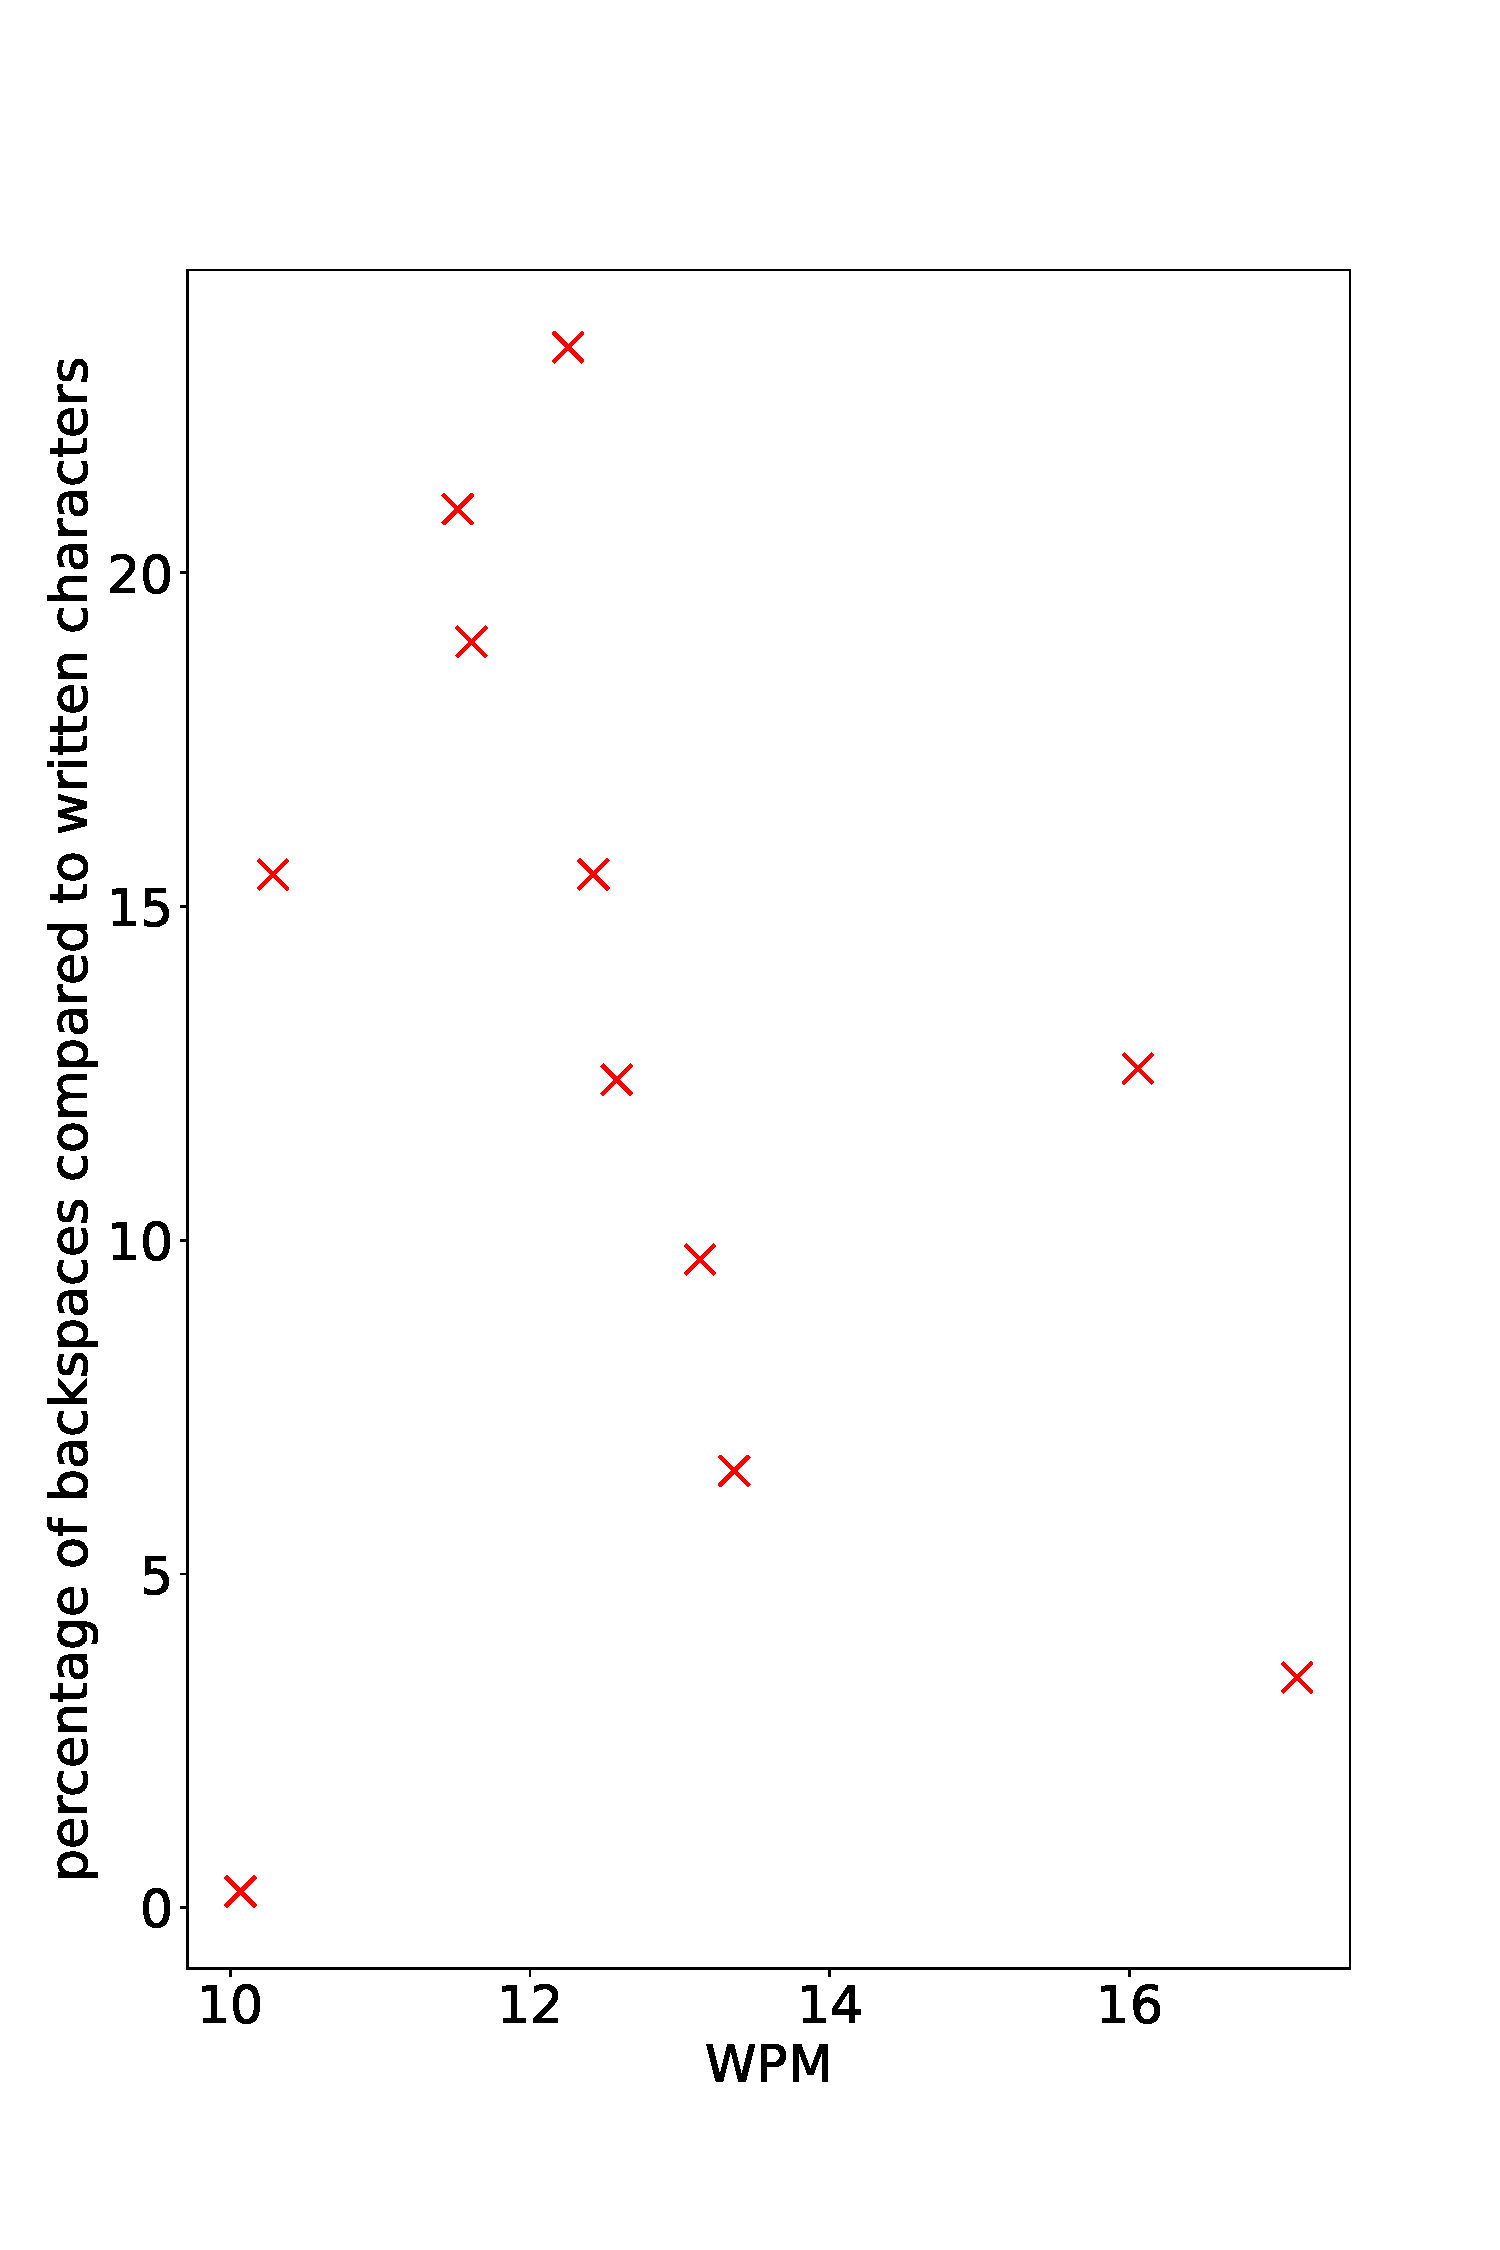
\includegraphics[width=0.5\textwidth]{backspace_error2.pdf}
    \caption{percentage of backspaces in relation to all characters in phrases compared to the wpm}
    \label{fig:error_backspace}
\end{figure}

In Fig \ref{fig:error_backspace} we show how many backspaces were used in relation to all written characters at which wpm value. We can not tell really much about it. But one thing that can be seen is, that the participant with the lowest wpm seemed to be very careful not overlooking wrong words that could be corrected by choosing the right suggestion. The participant with the highest wpm has the second-lowest percentual usage of backspaces. Therefore, they seem to get used to the system and its suggestions words very fast and good.\\
Overall, there seems to be a little trend, that participants with higher wpm values had to use fewer backspaces than participants with lower wpm values.\\

The next thing we want to calculate is the Total ER according to Soukoreff and MacKenzie \cite{10.1145/642611.642632}. First of all, we have to clarify, that we go for a bit of another approach regarding the transcribed text. In the Section \ref{sec:eva_task} we mentioned that the phrase, a participant wrote, had to match exactly the given phrase, otherwise it would not go to the next one. For the measure of the total ER value, we take the transcribed text as if a participant would not have been able to press the backspace. With only one exception, the backspace would have been allowed, if neither the best match nor the word suggestions had the right word and a wrong one is set. This means, the errors the participants did not correct immediately with the keyboard word suggestions count to the $INF$ value of the following formula: 

\begin{equation}
    Total\ ER = \frac{INF + IF}{C + INF + IF} \times 100\%
\end{equation}

Where $C$ is the number of correct keystrokes. Here we take the number of correct characters of each 15 phrases a participant had to input. $INF$ denotes the number of incorrect and not fixed characters in the transcribed text. For $INF$ we take from the words not corrected by a participant (with the transcribed text variant mentioned above). We do not count every character of such an error word as error, but we calculated the minimum string distance (MSD) between the error word and the word it should be. The MSD value is the number of single character insertions, deletions or substitutions to get from the wrong word to the right one. Finally, $IF$ denotes incorrect but fixed characters. We will set this value to 0, because for this calculation, we do not see it as an error, if a participant corrected the word immediately with a word suggestion from the keyboard. The following table shows our calculated results:
\label{sec:total_er}
\begin{table}[H]
    \centering
    \caption{Total ER per participant}
    \begin{tabular}{cc} \toprule
        participant&total ER\\ \midrule
        1&3.15\%\\
        2&2.95\%\\
        3&1.82\%\\
        4&2.26\%\\
        5&2.81\%\\
        6&2.18\%\\
        7&2.24\%\\
        8&1.69\%\\
        9&1.55\%\\
        10&0.53\%\\
        11&0\%\\\bottomrule
        average&1.93\%\\
        \bottomrule
    \end{tabular}
    \label{tab:wpm_compare}
\end{table}
As we can see in Table \ref{tab:wpm_compare}, the calculated total ER values are quite low. The averge is only 1.93\% with a standarddeviation of 0.93. Later, we will compare these values with others from another paper.\\

For the next calculation, we want to take a look at the not immediately corrected words together with the wpm. Firstly, we will do this with characters and then with the whole words. For the characters of an error word we take as in the previous calculation for the total ER the MSD values. Then we want to compare these with the same calculation, but without considering the errors happened because of ``the'', ``in'' and ``more''. We decide to remove these words, because they could be avoided through a small change in the best match calculations.
\begin{figure}[H]
    \makebox[\textwidth][c]{
        \centering
        \subbottom[Not corrected characters with wpm\label{fig:error_user:error_user1}]{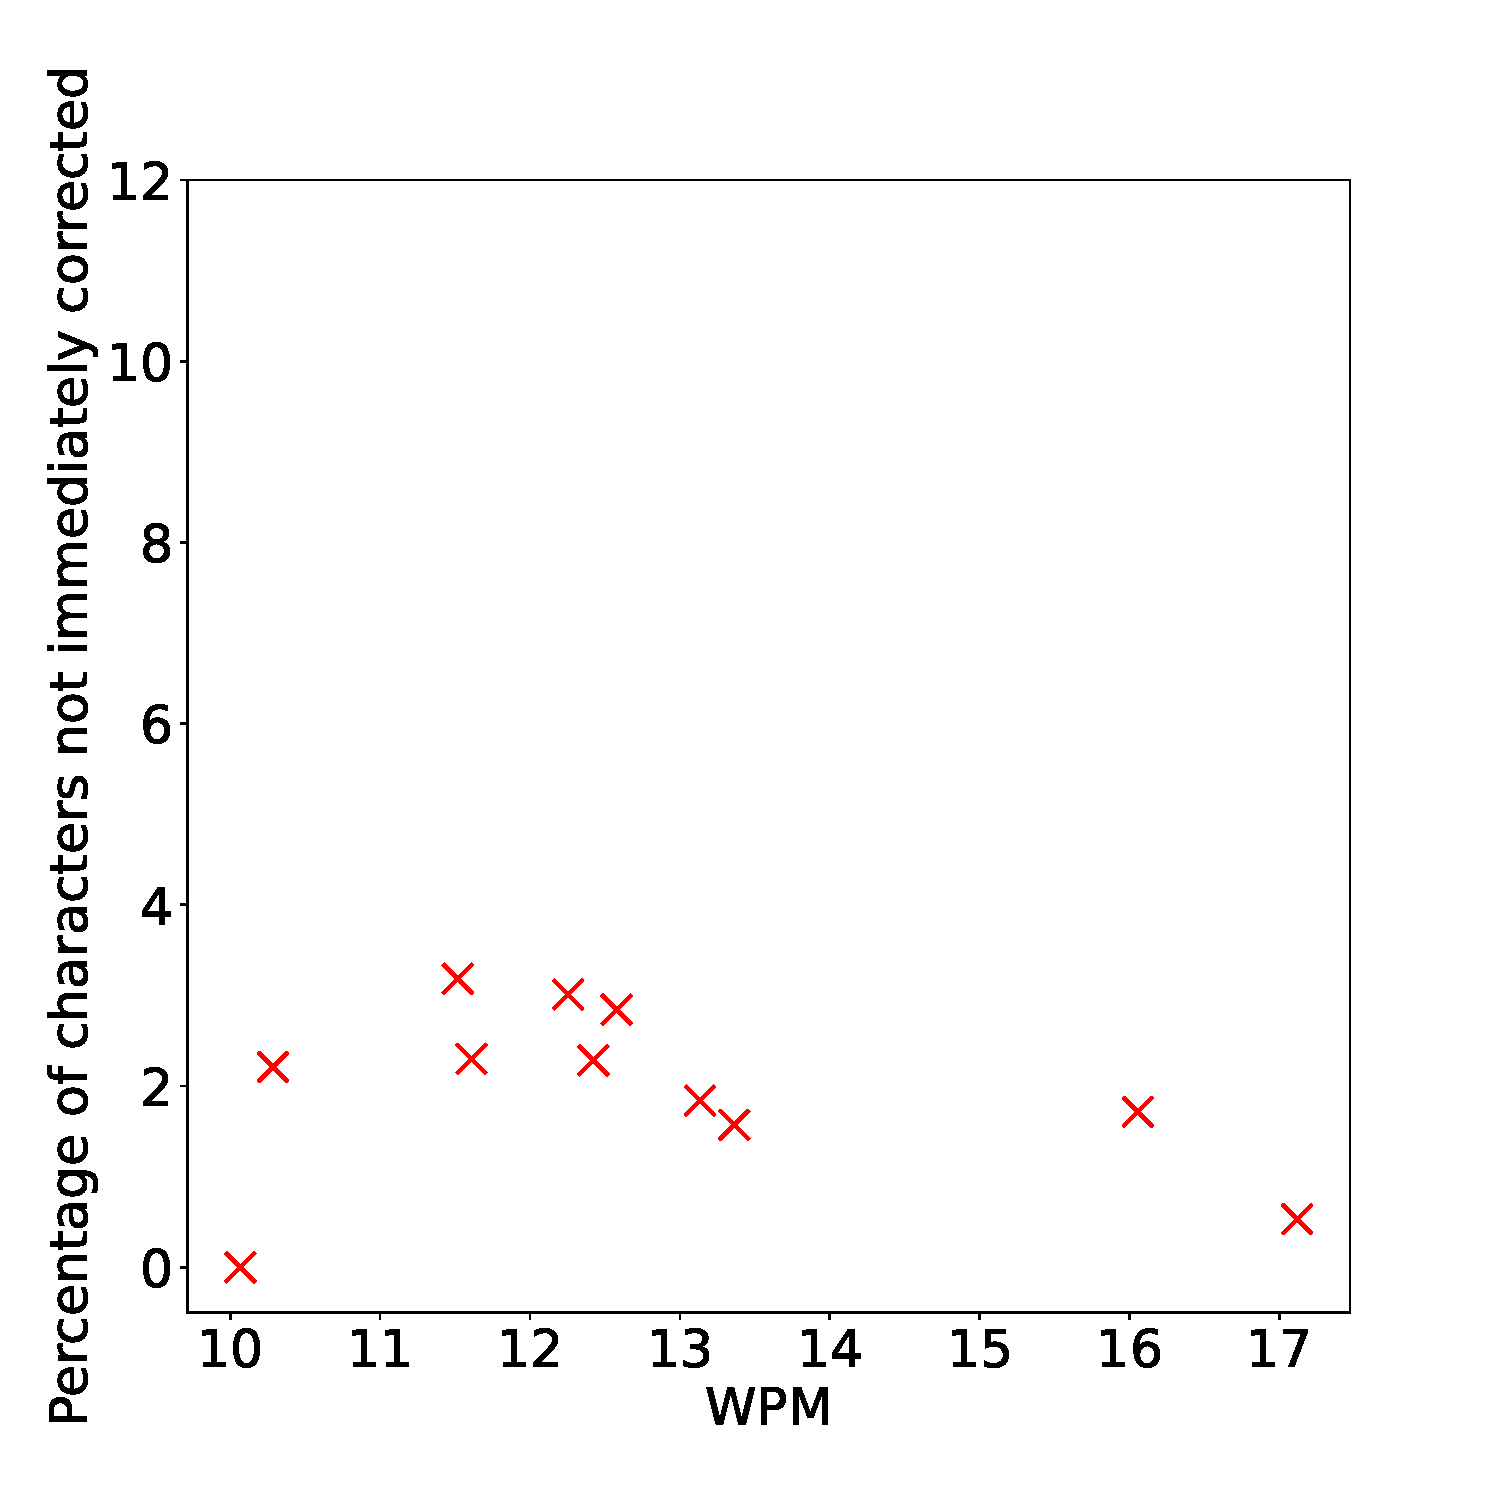
\includegraphics[width=0.6\textwidth]{user_error3_1.pdf}}\hspace{-3.0em}
        \subbottom[as (a), but without ``the'', ``in'' and ``more''\label{fig:error_user:error_user2}]{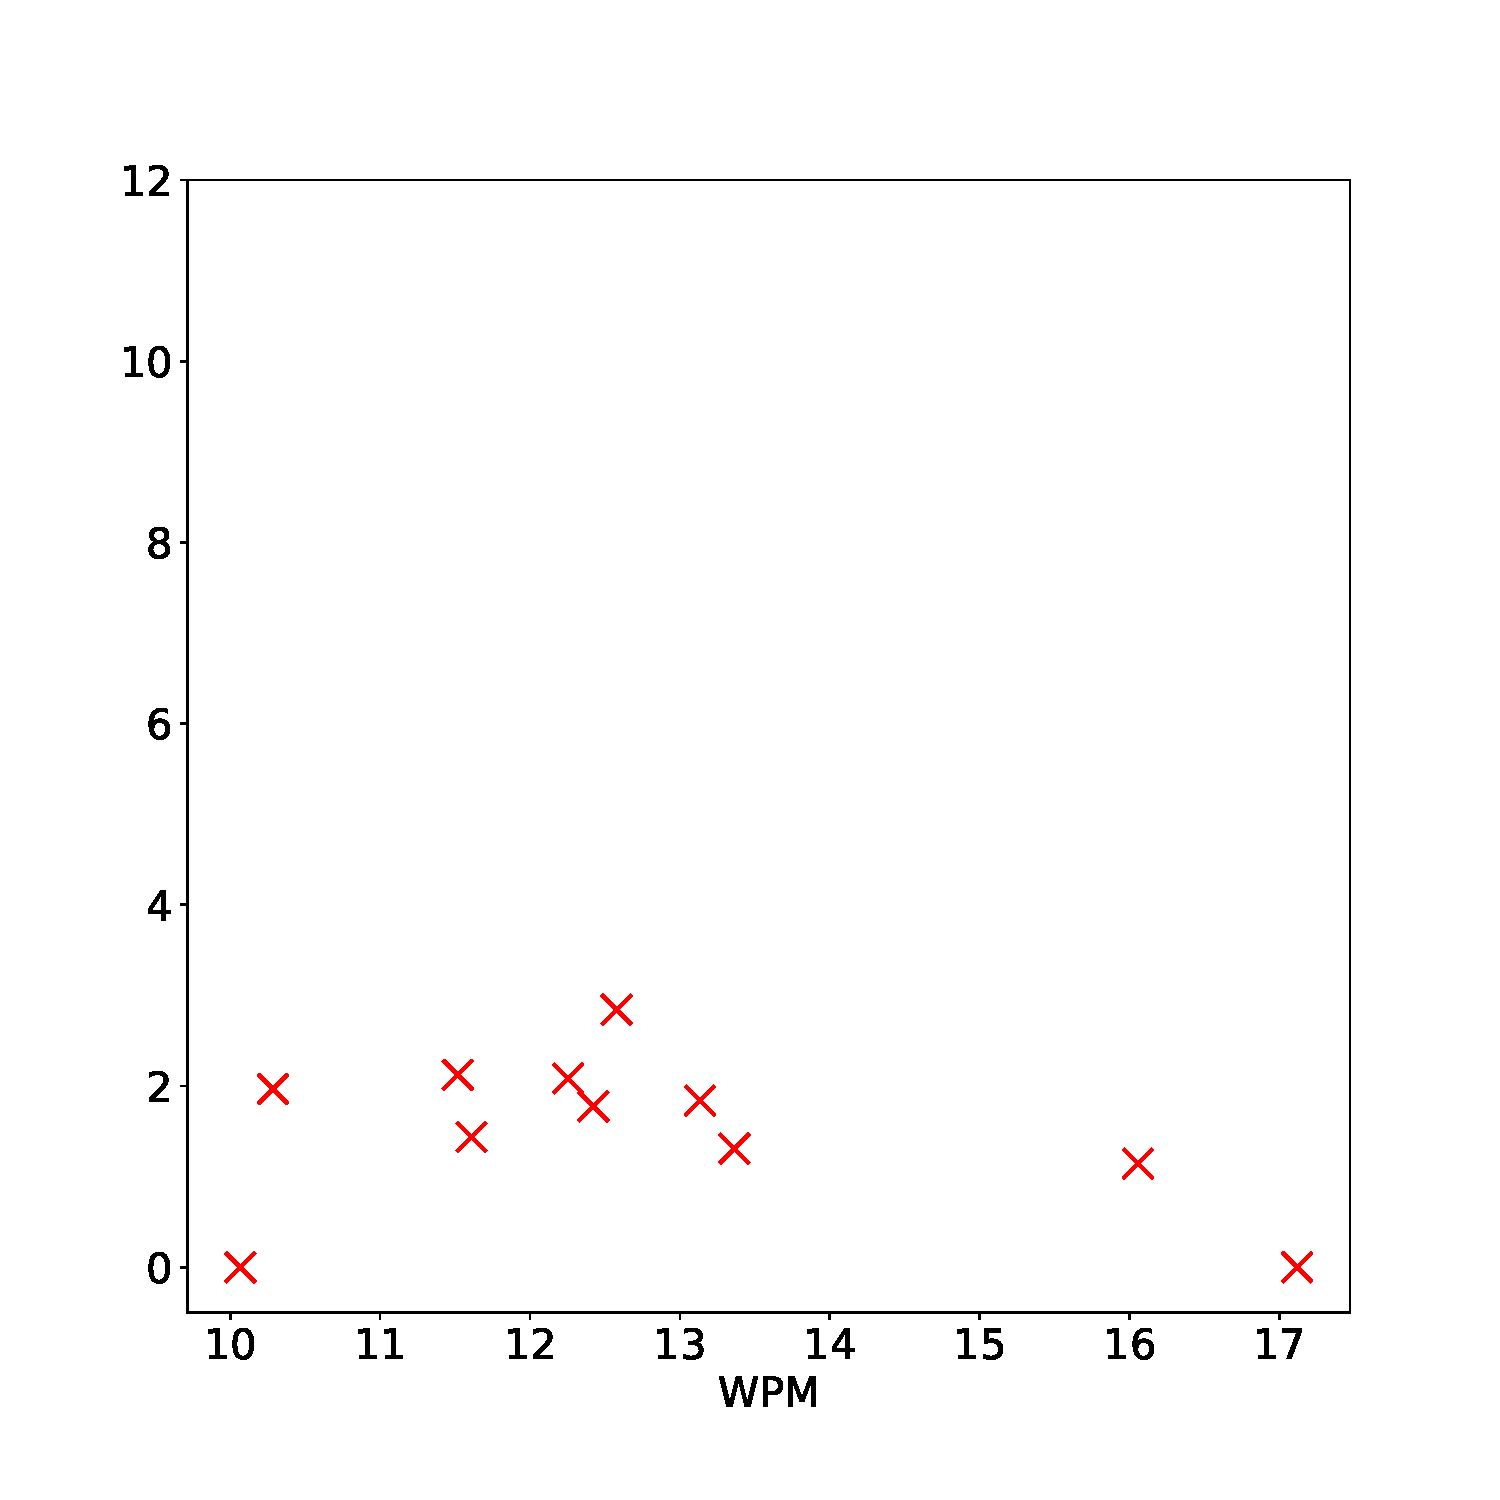
\includegraphics[width=0.6\textwidth]{user_error3_2.pdf}}
    }
    \makebox[\textwidth][c]{
        \centering
        \subbottom[Not corrected words with wpm\label{fig:error_user:error_user3}]{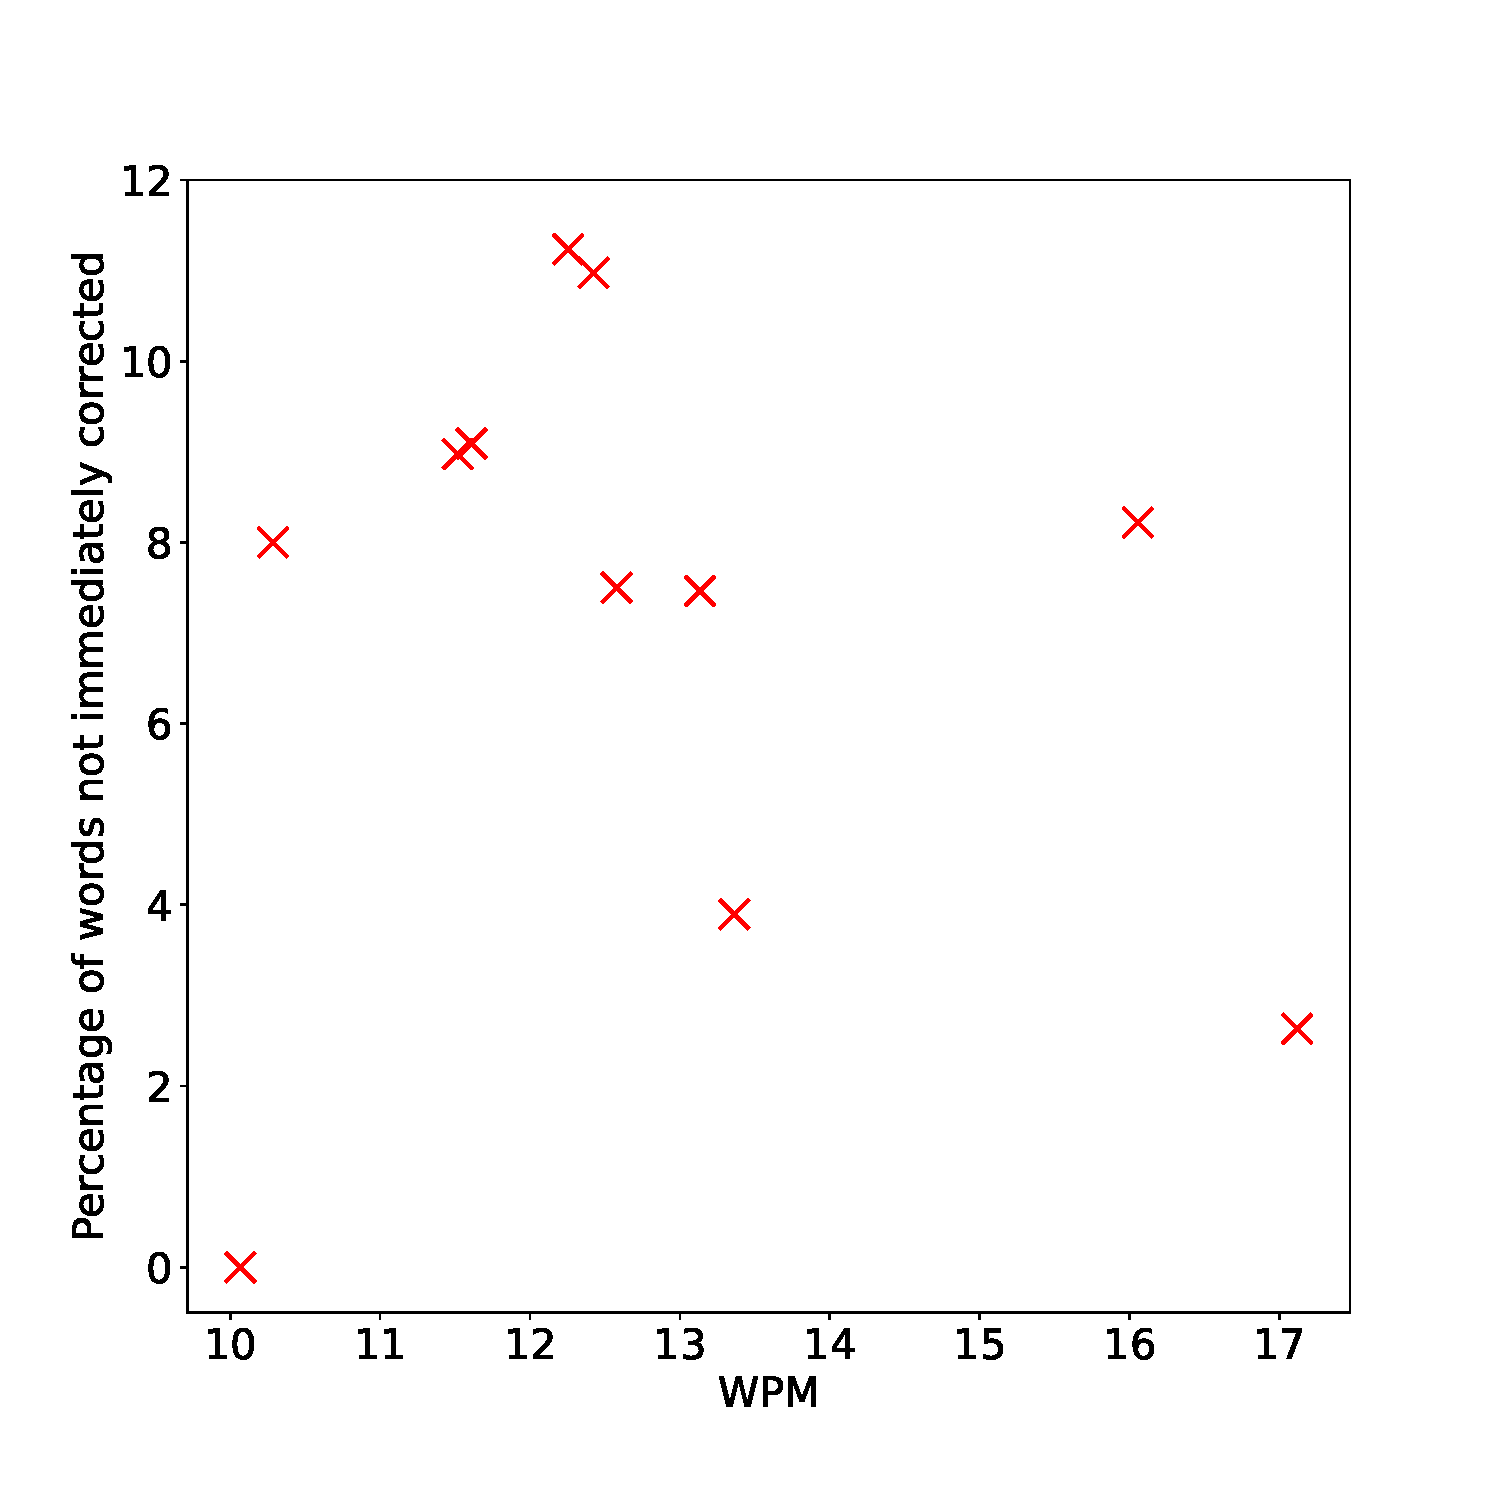
\includegraphics[width=0.6\textwidth]{user_error3_3.pdf}}\hspace{-3.0em}
        \subbottom[as (c), but without ``the'', ``in'' and ``more''\label{fig:error_user:error_user4}]{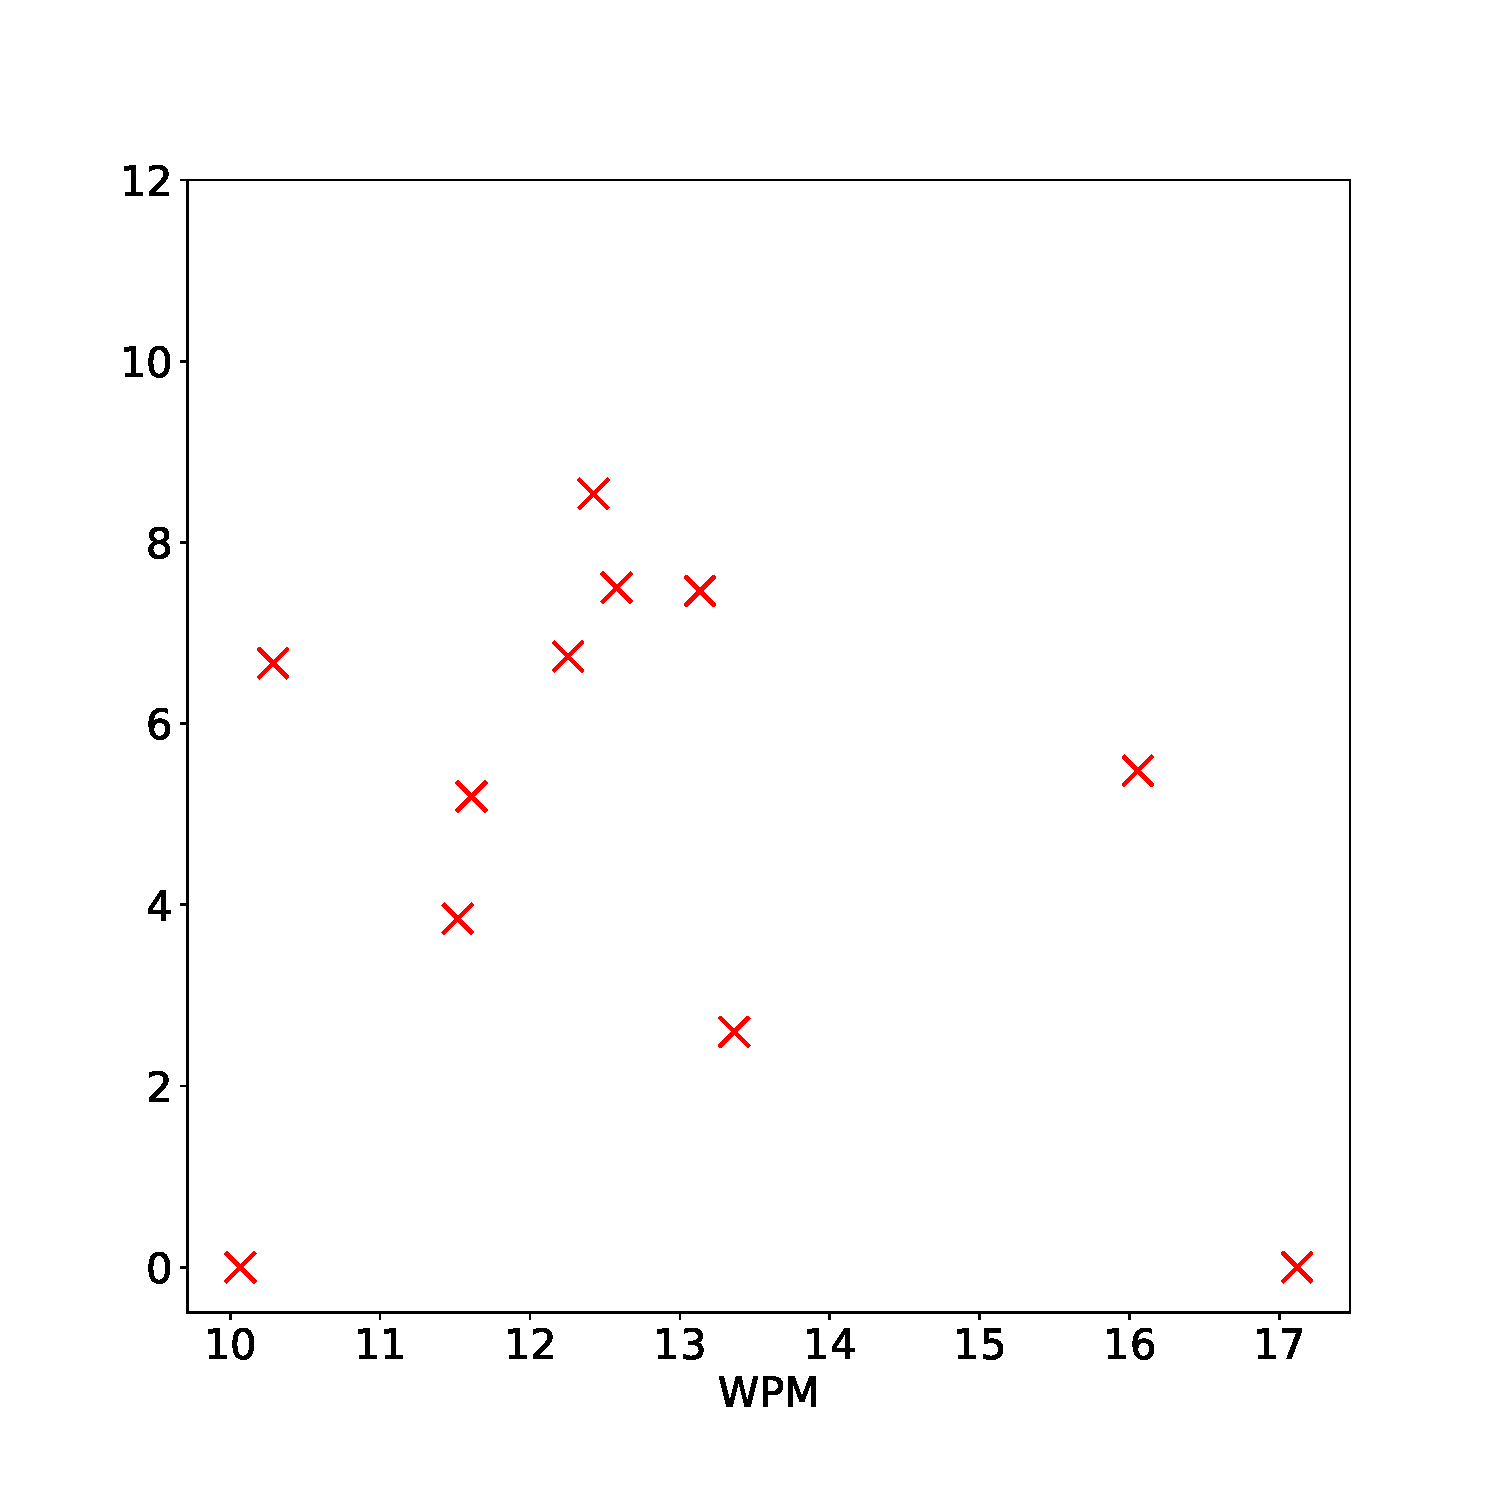
\includegraphics[width=0.6\textwidth]{user_error3_4.pdf}}
    }
    \caption{(a) shows the percentage of characters calculated with the MSD from wrong words, that are not immediately corrected with the word suggestions, (b) is the same as (a) but ``the'', ``in'' and ``more'' errors are ignored, (c) same as (a) but not with characters, but with the words as whole, (d) same as (b) but not with characters, but with the words as whole}
    \label{fig:error_user}
\end{figure}

In Fig \cref{fig:error_user:error_user1} and Fig \cref{fig:error_user:error_user2} we calculate the MSD of the words, a participant did not correct, although they had the chance to do it with the suggestions. On the y-axis, we look at the percentage, that these characters make up in comparison to all characters the participant had to write in all 15 phrases. In Fig \cref{fig:error_user:error_user1} we look at all wrong words. But a lot of the errors came from the words ``the'', ``in'' and ``more'', that could have been prevented as mentioned before. Therefore, in \cref{fig:error_user:error_user2} we look at the errors without considering these three words.\\
In the figures \cref{fig:error_user:error_user3} and \cref{fig:error_user:error_user4} we do the same, but without the MSD of the wrong words but just look at the number of them.\\
We can see, that the percentage of characters that are not corrected lies between about 0-4\%. For the words, the percentage of not corrected ones lies between 0\% and about 12\% which is much higher. This is because we work with the MSD. If a word is wrong, it will not be totally wrong and consist of similar letters as the right word. Therefore, not the whole word's characters will be counted into that value.\\
%One thing that can be observed is, that in the two lower figures of \Cref{fig:error_user} the percentage values are almost the same as in the two upper ones. This means that the words that were not corrected, have on average about the same length as the average length of all words from the respective 15 phrases is.\\
%One thing that can be observed at the left figures of Fig \Cref{fig:error_user} is that apart from one exception the percentage rate of not corrected words/characters is higher at lower wpm than it is at higher wpm. One obvious reason for this could be, that if words early in phrases were not corrected, a user had to delete the whole phrase back to the wrong word, and had to write all again. Therefore, it would make sense, that the faster participants made fewer errors, hence their risk of not correcting a word in the beginning of a phrase is lower. And then, they would not decrease their average wpm so much.
Another thing we can observe is, that the percentages drop quite an amount, if we ignore the ``the'', ``in'' and ``more'' errors.\\
To take another look at the participants' attention, we want to calculate the value of participant conscientiousness.

\subsubsection{Participant Conscientiousness}
As for the total ER, we also take the formula for the participant conscientiousness value from the paper of Soukoreff and MacKenzie \cite{10.1145/642611.642632}:
\begin{equation}
    Participant\ Conscientiousness = \frac{IF}{INF + IF}
\end{equation}

Normally, they would take the values of $IF$ and $INF$ as mentioned in Section \ref{sec:total_er}. We do either not really have $INF$ or $IF$. On one hand we can take the MSD of the not corrected words as $INF$ or on the other hand take the same value for $IF$, because the participant had to correct these words at one point.\\
To still get a value for the participant's conscientiousness we decide to work with words only, not characters. Thus, for $INF$ we count all the words not immediately corrected by a participant and for $IF$ the words that were corrected by using the keyboard's suggestions.\\
TODO: GRAPHICAL VISUALTISATION
A score of 100\% would be perfect. This would mean, that a participant corrects every word with the word suggestions, if it is possible. The average value we get here is 66.28\%, which means about two third of the words, that can be corrected with the suggestions, are corrected this way. The worst value is 33.33\% and the best value a participant achieved is 100\%. In our opinion, this score is not too bad. A lot of the participants are not used to word-gesture-keyboards and do not work or use VR that much. We think, if they used the keyboard over a longer period of time, they would get used to the words, that are sometimes harder for the keyboard to get as best match, and would pay more attention to use the word suggestions then.

\subsubsection{System Error Rate}
Here we do not want to see if a participant was paying attention or not, but rather if our algorithm finds the right words most of the time. We count all the words that were neither the best match nor in the word suggestions, such that a participant had no chance to get this word right the first time. If this happened multiple times to a word, we count it in every time.
\iffalse
\begin{figure}[H]
    \makebox[\textwidth][c]{
        \centering
        \subbottom[with characters\label{fig:error_system:error_system1}]{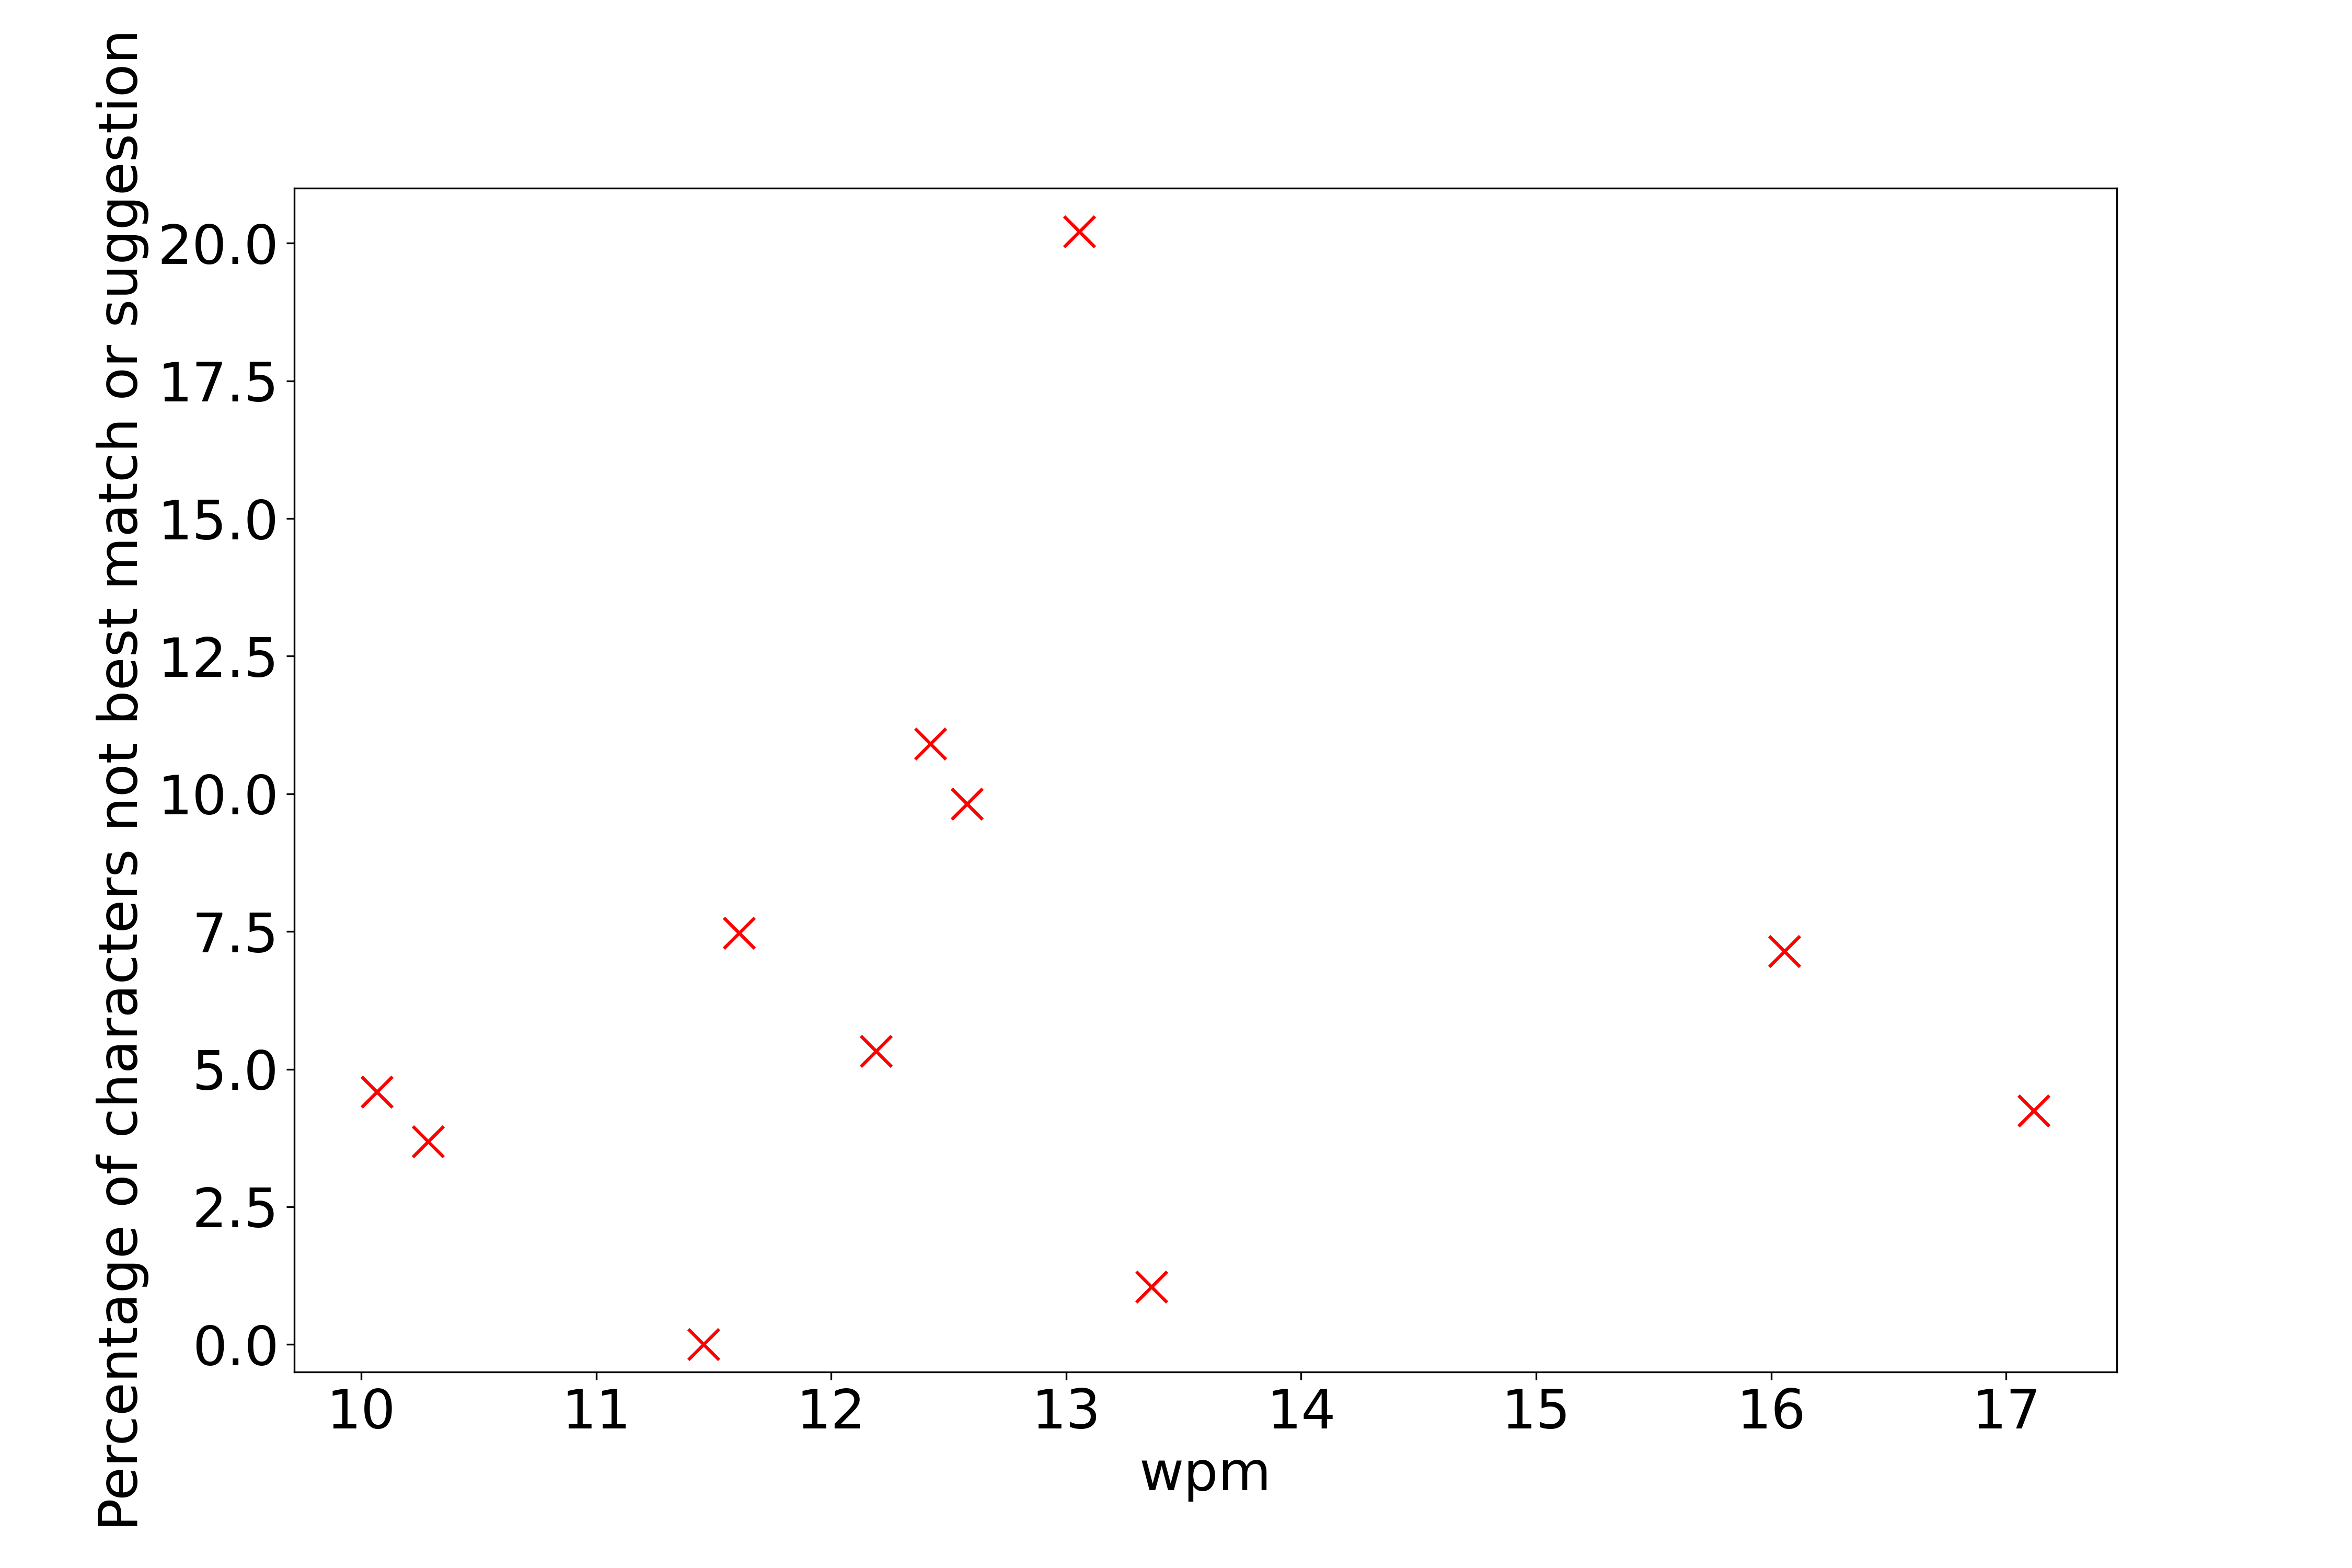
\includegraphics[width=0.6\textwidth]{system_error2_1.png}}\hspace{-3.0em}
        \subbottom[with words\label{fig:error_system:error_system2}]{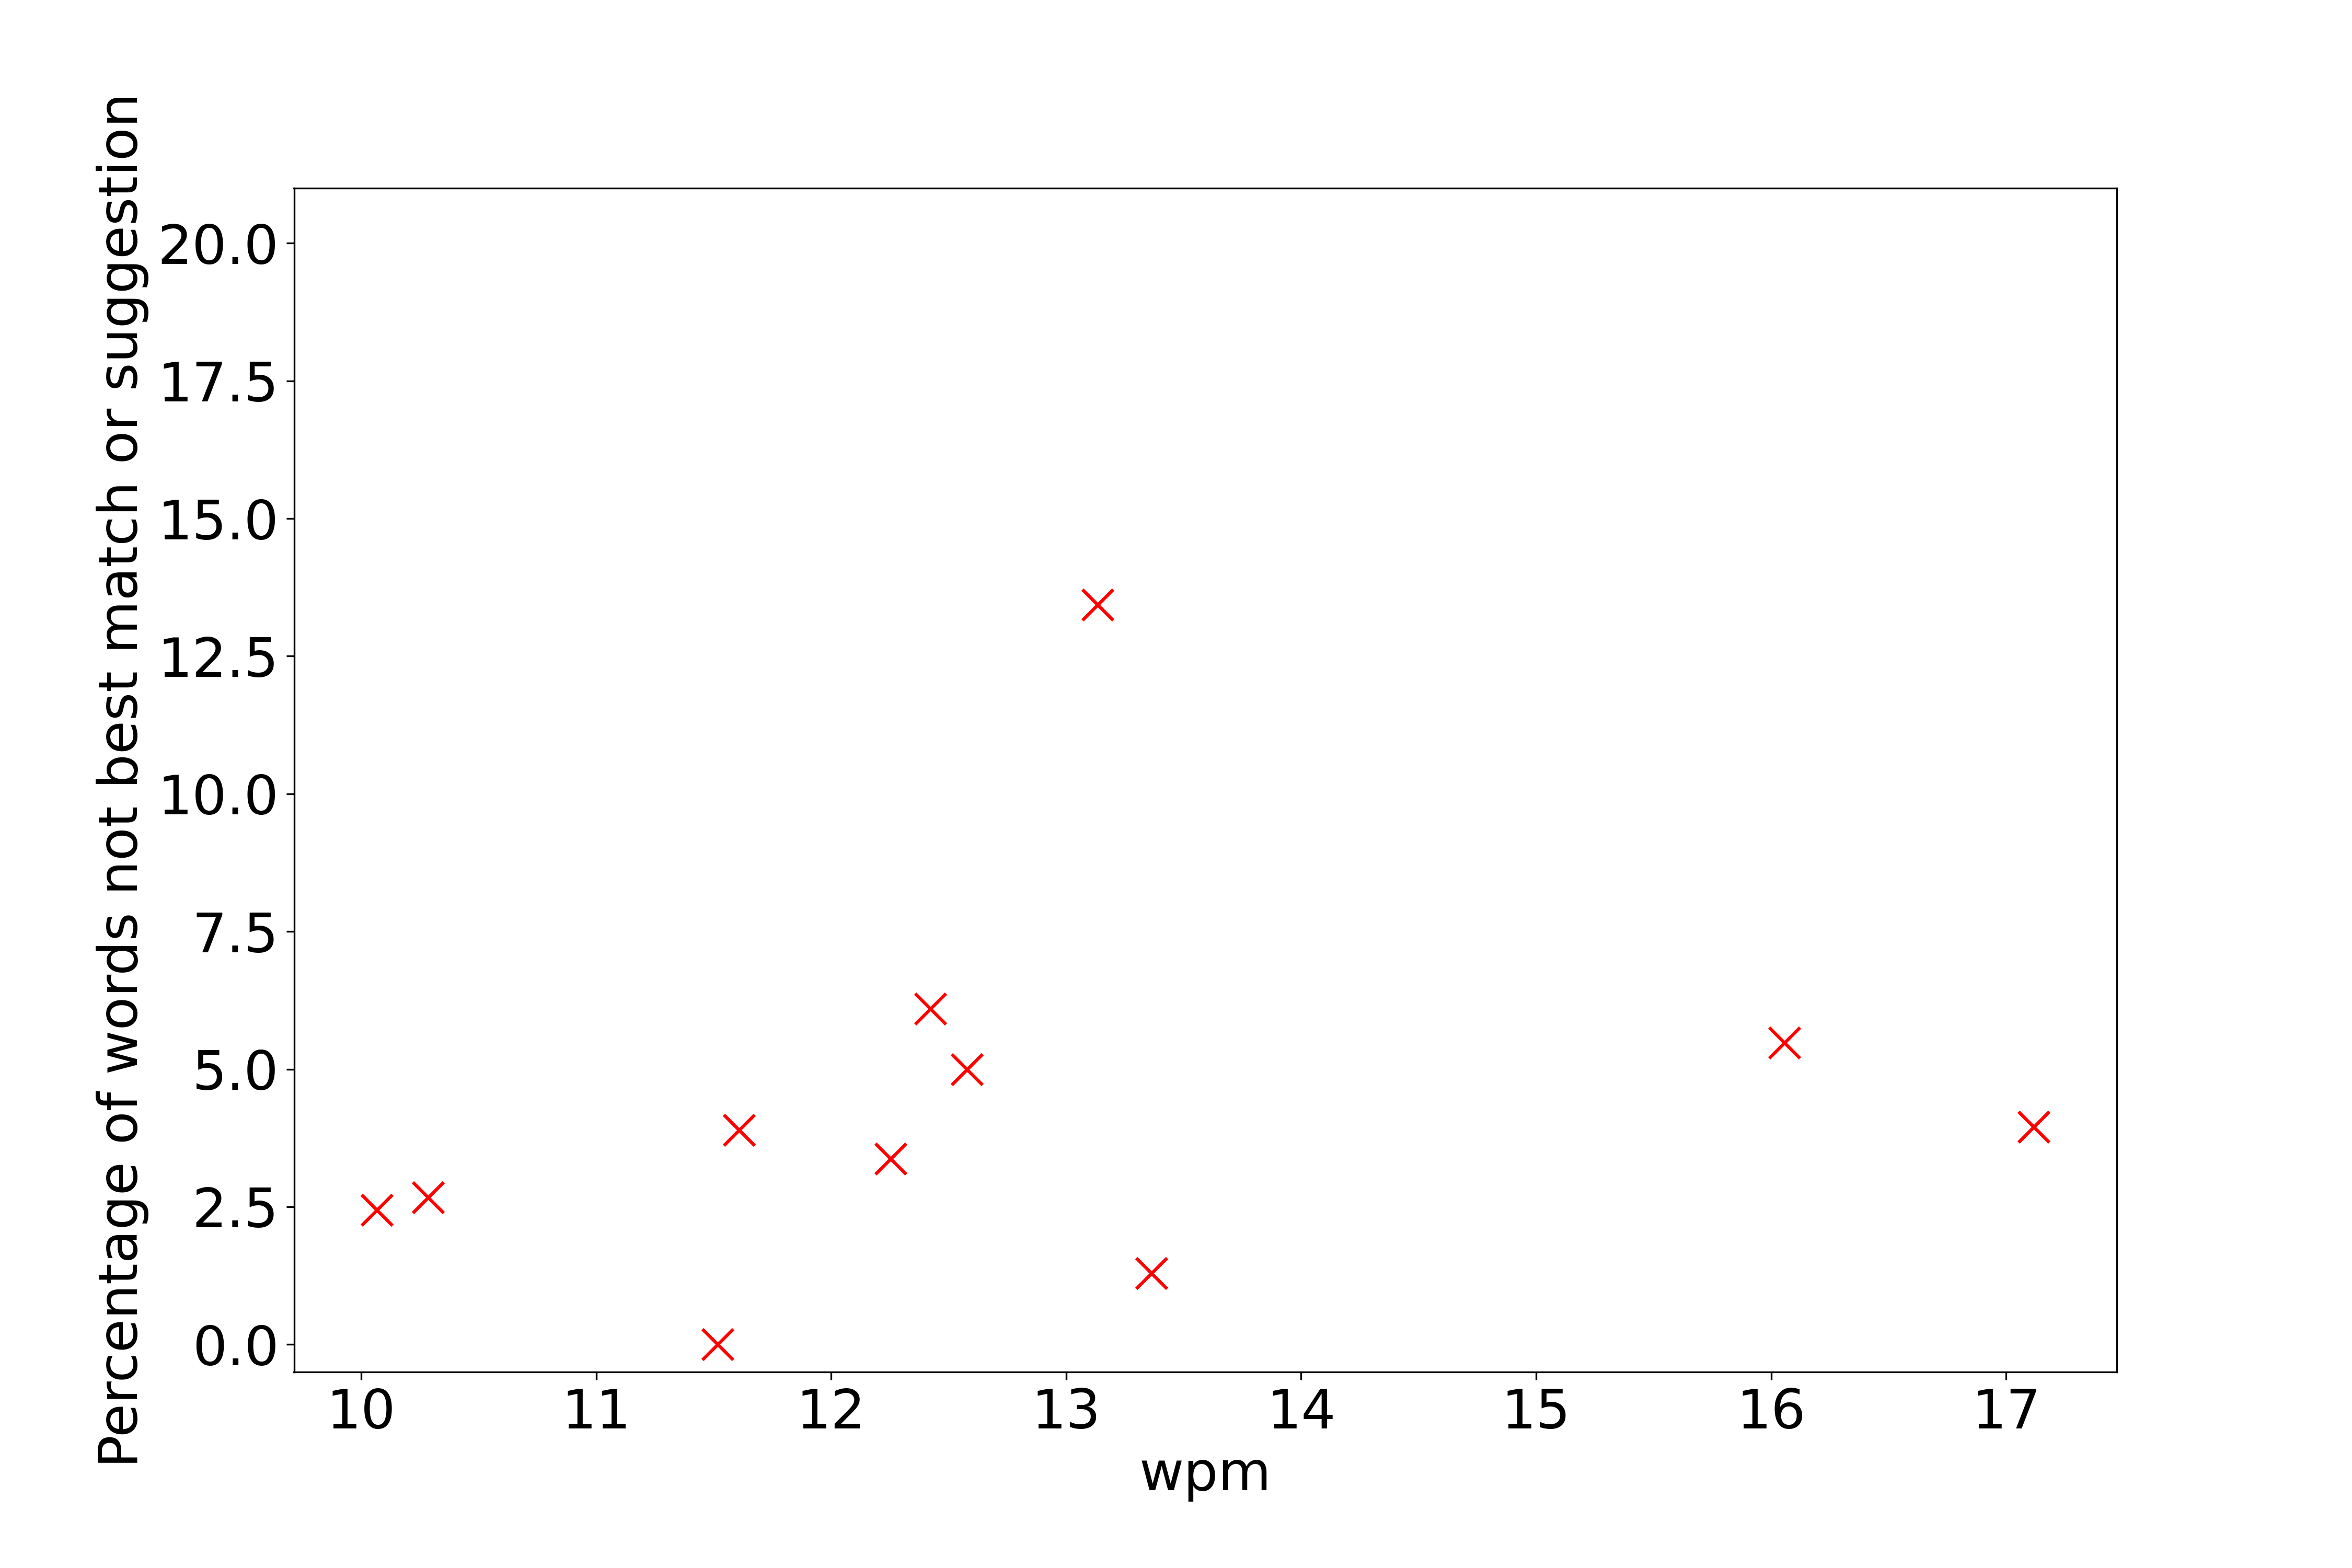
\includegraphics[width=0.6\textwidth]{system_error2_2.png}}
    }
    \caption{percentage of characters/words that were not found by the system neither as best match nor as suggestion}
    \label{fig:error_system}
\end{figure}
\fi

\begin{figure}[H]
    \centering
    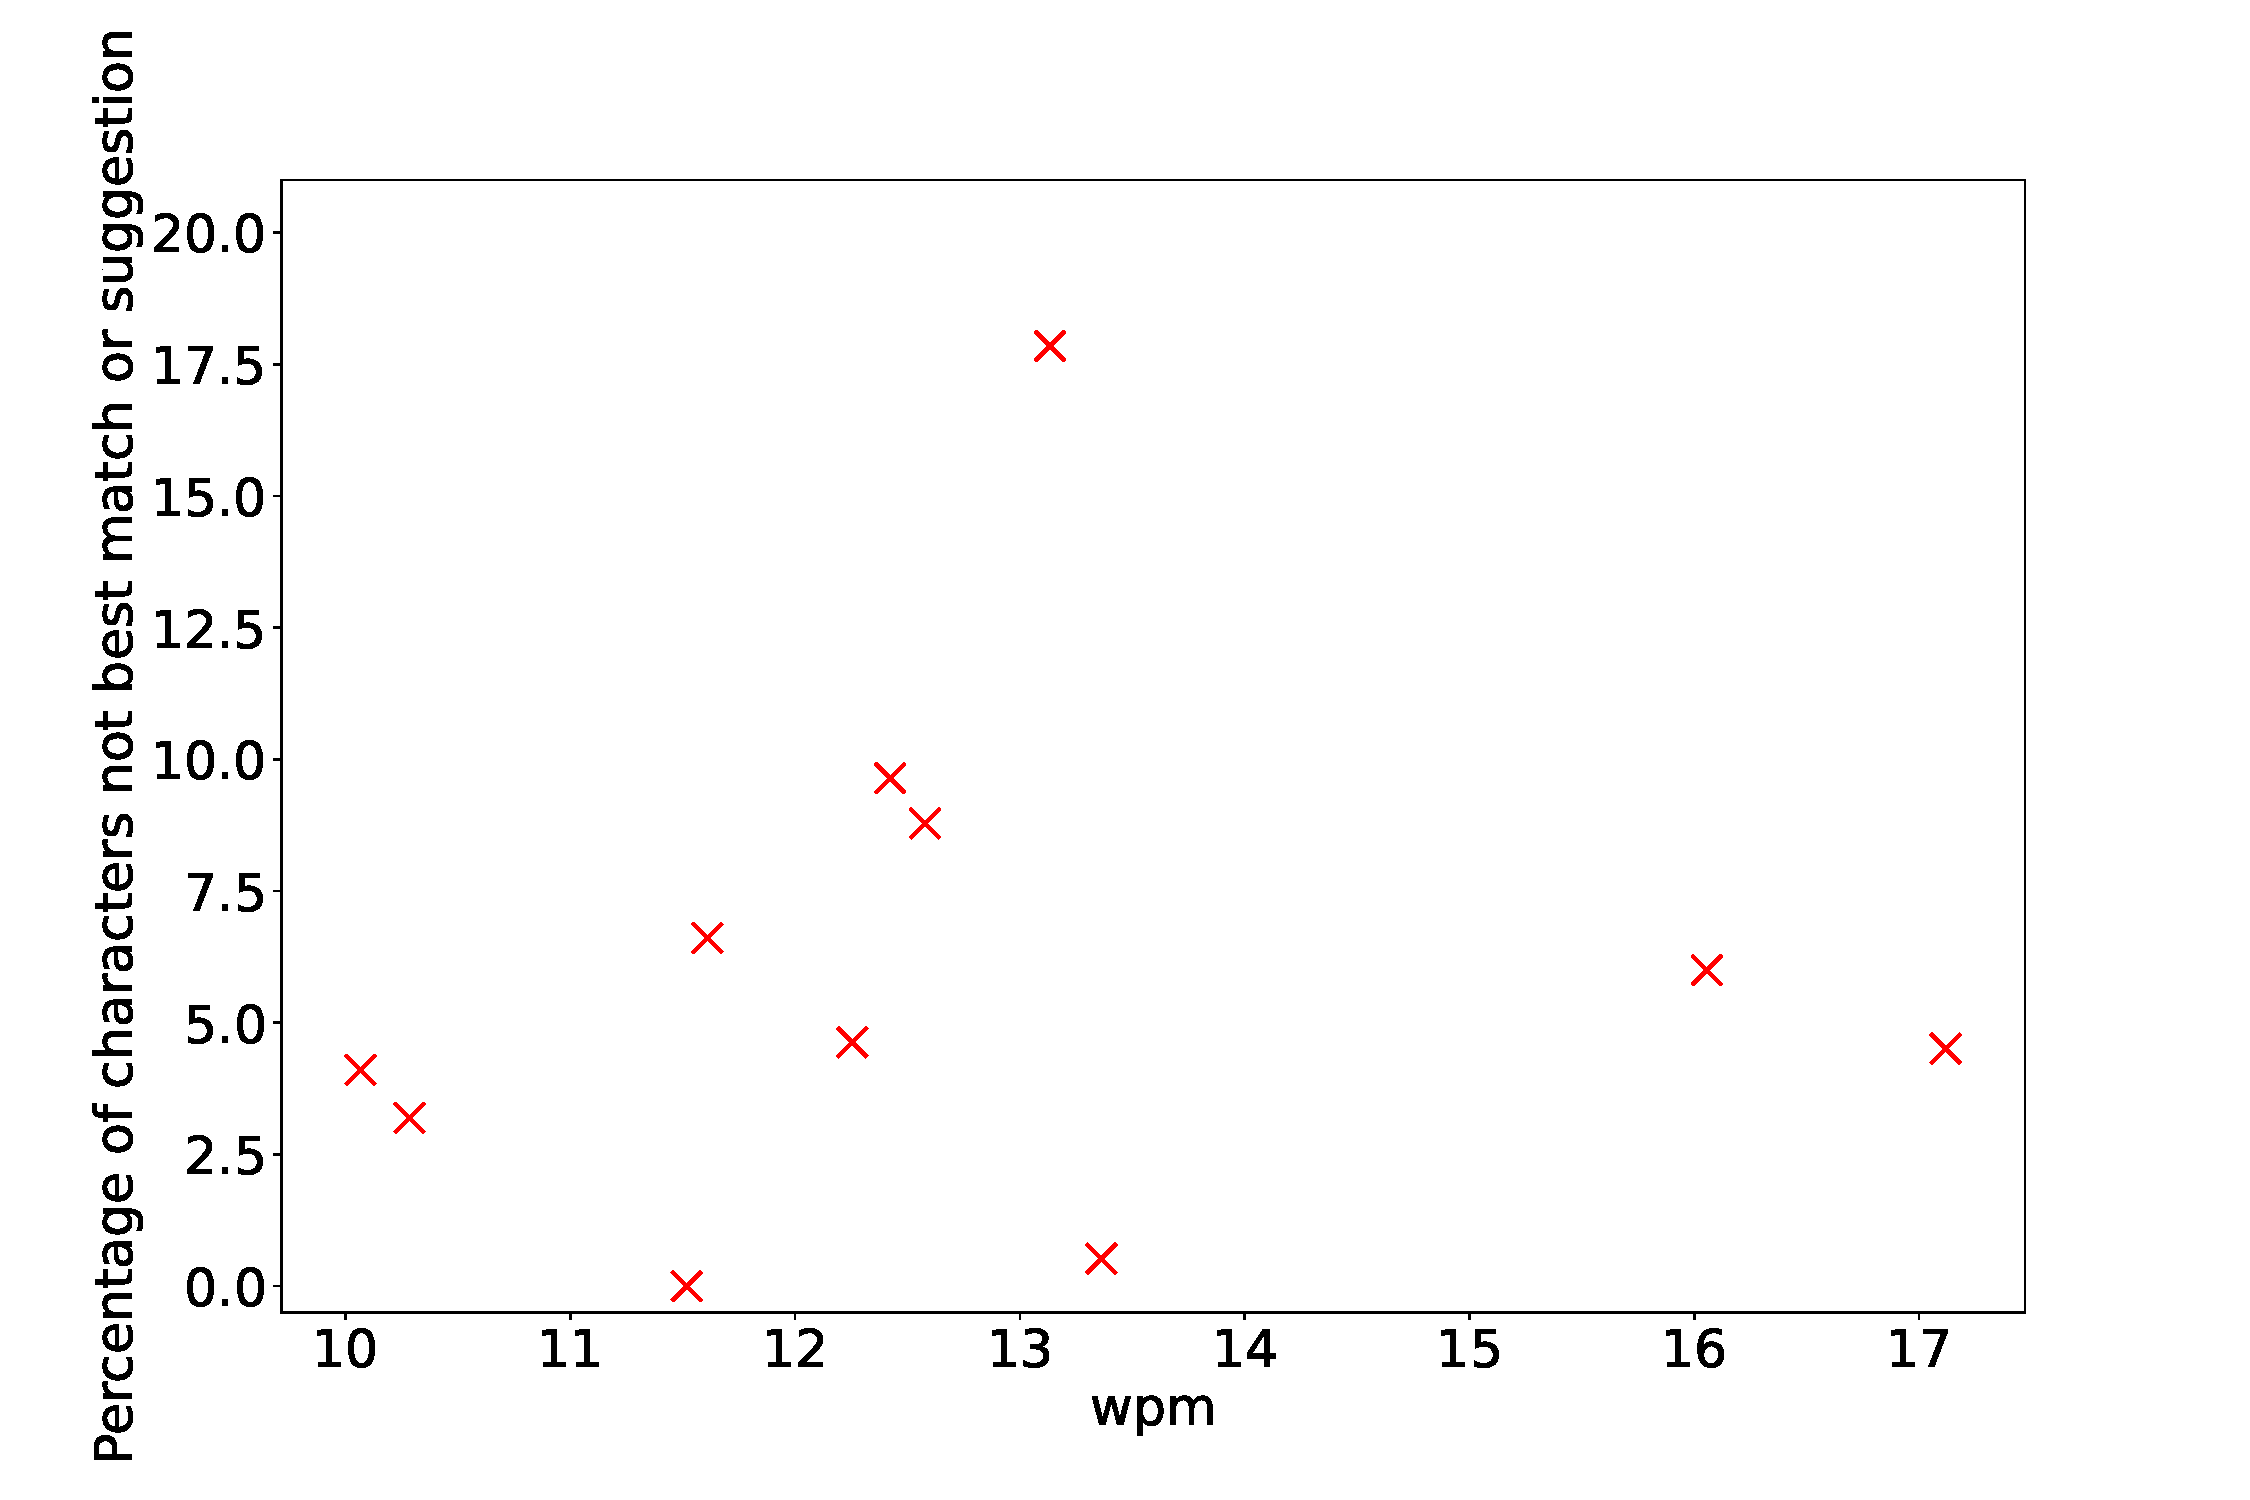
\includegraphics[width=0.8\textwidth]{system_error2_1.pdf}
    \caption{percentage of words that were not found by the system neither as best match nor as suggestion}
    \label{fig:error_system}
\end{figure}


In \Cref{fig:error_system} we can see what percentage of the words were not found by the system, neither directly as best match, nor as word suggestions, which a participant could choose it from. We decide to name this error the system error, although a participant could have done a really bad gesture which then would not really be the system's fault to not find a word.\\
We can see, that the percentage of words not found by the system, does not have a correlation with the wpm. We can not see a tendency, that either the ones with high wpm or the ones with low wpm have fewer problems with that.\\
On one hand, the average length of a word in the phrases we used is 4.16, on the other hand, the average length of a word the system has not found in the first try is 7.03. This tells us, that words with a length way bigger than the average one, are more error-prone. We think this makes sense, because the longer the word, most of the time, the longer the gesture. In a bigger gesture, deviations from the perfect graph are harder to prevent than in a small gesture.
%We can see, that in \cref{fig:error_system:error_system1} the percentages are much higher than in \cref{fig:error_system:error_system2}. This means that the words, which the system did not find a word, need to be longer than an average word in the written phrases. A reason for this might be, that often gestures for long words did not succeed. If a participant made some little curves too much in a gesture for a long word, the chances are lower, that the system can detect the right word, whereas for a small word the chance is higher, that the word gets found. Because the gesture can be much shorter and therefore fewer inaccuracies from a participant will happen.\\
%For the wpm and the percentages we can not detect any correlation. It seems, that these two values are not connected with each other. 

\subsection{Feedback}
The full list including all verbatim feedback from every participant can be found in the appendix. Here, we just want to highlight the most frequently addressed points.\\
Some participants find the best matches and suggestions sometimes confusing. The most mentioned example is that ``thee'' is preferred over ``the''.\\
The visualization of spaces or the current position are another thing that is frequently addressed. Some participants find it unclear where the cursor is, hence if a space is missing or not. They suggest to implement some kind of visual indication, that indicates, where the cursor currently is. We can say about this, that this problem existed in the evaluation environment, but in vitrivr-VR, the program that our keyboard is manly developed for, has these kinds of cursor visualization.\\
We also got a lot of praise and most of the time we saw a cheerful face when the VR headset got taken off. Some find it surprisingly intuitive, and others have a good feeling about using it.

\section{Discussion}
In this section we compare our results to other works' results and talk about some changes we did because of the feedback.

\subsection{Result Comparison}
First, we begin with the wpm. Boletsis and Kongsvik \cite{Boletsis2019ControllerbasedTT} evaluate in their paper four different VR input methods, a raycasting, drum-like, head-directed input and a split keyboard. The first one is a keyboard where a user can select letter by pointing a ray with a controller on it. For the second one the controllers simulate drum sticks in VR and letters have to be pressed by them. For the third keyboard a user has to aim with the head for the letters and press a button on the controller to input. The last keyboard is one, that is split into two halves, one assigned to each controller. 
\begin{table}[ht!]
    \centering
    \caption{wpm for different VR text input methods}
    \begin{tabular}{cc} \toprule
        text input method&wpm\\ \midrule
        Raycasting keyboard& 16.65\\
        Drum-like keyboard& 21.01\\
        Head-directed input keyboard& 10.83\\
        Split keyboard& 10.17\\
        Word-gesture keyboard& 12.75\\
        \bottomrule
    \end{tabular}
    \label{tab:wpm_compare}
\end{table}

In Table \ref{tab:wpm_compare} we listed the results of Boletsis and Kongsvik \cite{Boletsis2019ControllerbasedTT} and our measurement of the wpm value. They had a similar approach to the evaluation as we did, with one difference. They did use the same ten phrases for every participant and keyboard type.\\
As we can see, our keyboard lines up in the middle. It is not the one with the lowest wpm, but also not the one with the highest.

Another comparison we can do with the results of Boletsis and Kongsvik \cite{Boletsis2019ControllerbasedTT} is the total ER value.
\begin{table}[ht!]
    \centering
    \caption{total ER for different VR text input methods}
    \begin{tabular}{cc} \toprule
        text input method&wpm\\ \midrule
        Raycasting keyboard& 11.05\%\\
        Drum-like keyboard& 12.11\%\\
        Head-directed input keyboard& 10.15\%\\
        Split keyboard& 8.11\%\\
        Word-gesture keyboard& 2.14\%\\
        \bottomrule
    \end{tabular}
    \label{tab:total_er_compare}
\end{table}
The total ER for our keyboard seems to be much better than for the other input methods. A simple explanation could be that a user can make an error with every input. For the first four keyboards in \Cref{tab:total_er_compare} one input is equal to one character. Thus, if a user wants to input a phrase, they need to make inputs equal to the number of characters the phrase consists of. With a word-gesture keyboard, a user only has to make inputs equal to the amount of words in the phrase, which is usually much lower. And if the word is not the correct one, most of the time, it will not differ a lot from the word, that is intended to write. Therefore, in this case, there will not a lot of characters be added to the $INF$ value.

TODO: AVERAGE WPM FOR PERFECT SENTENCES

\subsection{New Implementations}
Because of the feedback and some observations, we decided to do one more implementations.\\
The first one is not a big change in code, but can still be pretty useful. We have the problem, that for example, ``thee'' is prioritized before ``the'', which does not make much sense, because ``the'' will be by far much more used in plain language. Because the word list we are currently using is ordered by the frequency of the words, we decided to let this influennce the best match and word suggestions. Now, if two or more words have the same highest score, the one that is highest in the word list will be taken, followed by the second highest and so on, until a word with a lower score comes next. This will prevent the problem with some words listed in Table \ref{tab:error_words}.